%%%%%%%%%%%%%%%%%% USAGE INSTRUCTIONS %%%%%%%%%%%%%%%%%%
% - Compile using LuaLaTeX and biber, unless there is a particular reason not to. Do not use the older LaTex/PDFLaTeX or BibTeX. (The fonts won't work correctly.)
% - Expect to get 2 warnings when working correctly, one on xcolor and hyperref, and one on ExtSizes saying is better to use a class. These can be ignored.
% - Font and the report 'year' must be specified when all \documentclass or the template won't work correctly. (There's no error checking/default cases!)
% - For best performance save images/graphics as PDF files, not as png/jpg/eps. This makes no difference to how images are inserted using \includegraphics.
% - As many further packages as wanted can be loaded. Below are just an example set. Note that template itself loads a number of packages, including hyperref.
% - References are handed using biblatex.
% - Link to the presentation of dissertations policy: https://documents.manchester.ac.uk/display.aspx?DocID=2863



%%%%%%%%%%%%%%%%%% META DATA SETUP %%%%%%%%%%%%%%%%%%
% This is where the document title and author are set. Other details for the title page are set later
% Note that if/when you edit these you may need to 'Recompile from scratch' to get the changes to display in the PDF. (In Overleaf, select the down arrow to the right of the 'Recompile' button)
\begin{filecontents*}{\jobname.xmpdata}
	\Title{Energy-Efficient UAV Path Planning in IOT Networks: A
		Deep Reinforcement Learning Aided Approach} 
	\Author{11085980} % should be student number rather than name to help with annoymous marking
	\Language{en-GB}
	\Copyrighted{True}
	% More meta-data fielda can be added here if wanted, see https://ctan.org/pkg/pdfx?lang=en for fields
\end{filecontents*}


%%%%%%%%%%%%%%%%%% DOCUMENT SETUP %%%%%%%%%%%%%%%%%%
\documentclass[12pt,beng]{uom_eee_dissertation_casson} % course can be msc or beng
% Check your course handbook for the correct font size to use. Make sure this is correct - you may get an overlength penalty if not! Is currently 12 for BEng, and 11 for MSc. The template doesn't change this automatically for you


%%%%%%%%%%%%%%%%%% PACKAGES AND COMMANDS %%%%%%%%%%%%%%%%%%

% Packages
\usepackage{graphicx}              % for adding graphics files
\graphicspath{
  {./images/}
  {../src/agents/dqn/dqn_evaluation_results/multi_seed_results/}
  {../src/agents/dqn/dqn_evaluation_results/baseline_results/}
  {../src/agents/dqn/dqn_evaluation_results/sweep_fairness_results/}
  {../src/agents/dqn/dqn_evaluation_results/ablation_results/}
  {../src/agents/dqn/dqn_evaluation_results/trajectory_results/}
  {../src/agents/dqn/dqn_evaluation_results/sim_to_real_results/}
  {../src/agents/dqn/dqn_evaluation_results/cross_layout_results/}
  {../src/agents/dqn/dqn_evaluation_results/training_results/}
}
\usepackage{amsmath}               % assumes amsmath package installed
\allowdisplaybreaks[1]           % allow eqnarrays to break across pages
\usepackage{amssymb}               % assumes amsmath package installed 
\usepackage{url}                   % format hyperlinks correctly
\usepackage{rotating}              % allow portrait figures and tables
\usepackage{multirow}              % allows merging of rows in tables
\usepackage{lscape}                % allows pages to be typeset in landscape mode
\usepackage{tabularx}              % allows fixed width tables
\usepackage{verbatim}              % enhanced version of built-in verbatim environment
\usepackage{footnote}              % allows more control over footnote environments
\usepackage{float}                 % allows H option on floats to force here placement
\usepackage{booktabs}              % improve table line spacing
\usepackage{lipsum}                % for adding dummy text here
\usepackage[base]{babel}           % required for lisum package
\usepackage{subcaption}            % for multiple sub-figures in a single float
\usepackage{siunitx}               % add SI units
\usepackage{algorithm}             % for algorithm floats
\usepackage{algpseudocode}         % for algorithmic pseudocode
\usepackage{listings}              % for \lstinline inline code formatting
% TikZ for inline diagrams
\usepackage{tikz}
\usetikzlibrary{arrows.meta, shapes.geometric, positioning, calc,
                decorations.markings, decorations.pathmorphing,
                backgrounds, fit}

% Override class font: use Calibri directly (installed on Windows via Office)
% Placed last in preamble so it overrides the class's \setmainfont{Carlito}
\setmainfont[
  Ligatures=TeX,
  BoldFont={Calibri Bold},
  ItalicFont={Calibri Italic},
  BoldItalicFont={Calibri Bold Italic}
]{Calibri}

% Make \includegraphics tolerant of missing files during drafting:
% if the file is absent, render a visible placeholder box and continue
% the compile rather than halting.
\usepackage{xcolor}
\let\uomorigincludegraphics\includegraphics
\renewcommand{\includegraphics}[2][]{%
  \IfFileExists{#2}%
    {\uomorigincludegraphics[#1]{#2}}%
    {\fbox{\parbox{0.6\linewidth}{\centering\vspace{1em}%
      \textbf{\color{red!70!black}[Missing figure]}\\[2pt]%
      {\footnotesize\ttfamily\detokenize{#2}}\vspace{1em}}}}%
}

% Override the UoM class's uomappendix environment so the appendices render
% as a single numbered "A Appendices" section with A.1 ... A.N subsections,
% matching the Y3 project template used across the cohort.
\renewenvironment{uomappendix}{%
  \clearpage
  \bookmarksetupnext{level=-1}%
  \addtocontents{toc}{\protect\setcounter{tocdepth}{2}}%
  \begin{appendices}%
    \section{Appendices}%
}{%
  \end{appendices}%
}

% Custom commands
\newcommand{\degree}{\ensuremath{^\circ}}
\newcommand{\sus}[1]{$^{\mbox{\scriptsize #1}}$} % superscript in text (e.g. 1st)
\newcommand{\sub}[1]{$_{\mbox{\scriptsize #1}}$} % subscript in text
\newcommand{\otoprule}{\midrule[\heavyrulewidth]}
\newcolumntype{Z}{>{\centering\arraybackslash}X}  % tabularx centered columns 
% Add your custom commands here

% Handbook §9.2: text must be left-aligned throughout (incl. abstract, front matter)
\AtBeginDocument{\raggedright}


%%%%%%%%%%%%%%%%%% REFERENCES SETUP %%%%%%%%%%%%%%%%%%

% Setup your references here. Change the reference style here if wanted
\usepackage[style=ieee,backend=biber,backref=true,hyperref=auto,maxbibnames=3,minbibnames=1]{biblatex}
% Note backref=true adds a page number (and hyperlink) to each reference so you can easily go back from the references to the main document. You may prefer backref=false if you need to stick strictly to a given reference style


% Fixes which can't be applied in the .cls file
\DefineBibliographyStrings{english}{backrefpage = {cited on p\adddot},  backrefpages = {cited on pp\adddot}}
%  \renewcommand*{\bibfont}{\large}


% Add more .bib files here if wanted
\addbibresource{references.bib}



%%%%%%%%%%%%%%%%%% AUTOMATIC WORD COUNT SETUP %%%%%%%%%%%%%%%%%%
% Automatically counts the words present and makes a \mywordcount variable. This is used later to automatically add the word count (which can be overridden if wanted)
% See https://www.overleaf.com/learn/how-to/Is_there_a_way_to_run_a_word_count_that_doesn%27t_include_LaTeX_commands%3F for info on what words are counted and how to control this. Any changes to what's counted need to be made in uom_thesis_casson.cls, in the \newcommand{\quickwordcount} command. The default doesn't count words in headings, captions, or references and so you may get slightly different numbers if use a different word count tool
% This can be a bit fragile. If it doesn't work, there's an option later on to just type in a numer
%\quickwordcount{\currfilebase} % run word count. This just counts the words. Is displayed with the \wordcount command later



%%%%%%%%%%%%%%%%%% START DOCUMENT %%%%%%%%%%%%%%%%%%

% Don't edit these lines, title and author are automatically taken from the document meta-data defined above
\begin{document}
	\makeatletter
	\title{Energy-Efficient UAV Path Planning in IOT Networks: A
		Deep Reinforcement Learning Aided Approach}
	\studentid{11085980}
	\makeatother
	
	% Set the below yourself
	\course{Electrical and Electronics Engineering}    % BEng course
	\faculty{Science and Engineering}                  % "Faculty of" is added automatically
	\school{School of Engineering}
	\submitdate{2026}                                  % regulations ask only for the year, not month
	\wordcount{12537}		                   % use \wordcount{} to set the count. Can just type in a number (e.g. \wordcount{1000}	if don't want to use the automatic count.) This is automatically displayed after the table of contents.
	\maketitle
	
	
	
	%%%%%%%%%%%%%%%%%% LISTS OF CONTENT %%%%%%%%%%%%%%%%%%
	\uomtoc
	% other lists are not required, but can include \uomlof and \uomlot if really want to
	
	
	%%%%%%%%%%%%%%%%%% ABSTRACT %%%%%%%%%%%%%%%%%%
	\begin{abstract} % put abstract here.
        This dissertation addresses energy-efficient, dynamic path planning for Unmanned Aerial
Vehicles (UAVs) tasked with data collection in unsynchronised LoRaWAN Internet of Things
(IoT) networks. The integration of mobile UAV gateways into LoRaWAN introduces a fundamental
challenge: rapid link-quality changes caused by UAV movement drive devices to converge on
identical Spreading Factors, collapsing packet delivery rates in a phenomenon termed the
``SF Monoculture.''

We propose a protocol-aware Deep Reinforcement Learning (DRL) framework, utilising a
Deep Q-Network (DQN) agent trained within a custom, high-fidelity Gymnasium environment.
The environment models the UAV's position as a direct control input to the LoRaWAN protocol,
incorporating the Two-Ray Ground Reflection path loss model, log-normal shadowing, EMA-based
Adaptive Data Rate (ADR) latency, asynchronous duty cycles, and the LoRa Capture Effect.
A Domain Randomisation and Curriculum Learning regime produces a single generalised policy,
deployable without retraining across grids spanning $100 \times 100$ to $1{,}000 \times 1{,}000$
cells and network densities of 10 to 40 sensors.

Rigorous evaluation over five independent random seeds and multiple network configurations
demonstrates that the DQN agent consistently outperforms both a protocol-blind Nearest-Sensor
Greedy and a novel SF-Aware Max-Throughput Greedy baseline. At 40 sensors, the DQN achieves
a Jain's Fairness Index of $0.672 \pm 0.054$ versus $0.646 \pm 0.053$ for the SF-Aware
baseline (+4.0\%) and $0.664 \pm 0.055$ for the Nearest baseline (+1.2\%), with a $+7.3\%$
improvement in energy efficiency (bytes per watt-hour). The DQN's advantage is statistically
significant ($p < 0.05$, Welch's $t$-test) at compact operational scales, and grows
monotonically with network density. The key emergent behaviour is strategic repositioning:
the DQN uniquely allocates 2.9\% of steps to deliberate movement ($p = 0.002$, Welch's
$t$-test), reaching positions that yield $+14\%$ more bytes per collection step than
greedy baselines---demonstrating that the UAV's physical position can serve as an active
control variable for the communication protocol.

	\end{abstract}%
	% Note: the abstract environment already issues \clearpage; no extra one needed here.


	%%%%%%%%%%%%%%%%%% DECLARATIONS %%%%%%%%%%%%%%%%%%
	\begin{uomoriginality}
		\uomoriginalitydeclaration 
		% If the standard originality decalaration is sufficient, saying no portion of the work has been submitted in support of an application for another degree or qualification, the above command will automatically add the required text and nothing else is needed in this section.
		% If the standard statment isn't sufficient, then comment out the \uomoriginalitydeclaration command and type in your own text here explaining the authorship of any re-used portions. 
	\end{uomoriginality}
	\uomcopyrightstatement
	
	
	
	%%%%%%%%%%%%%%%%%% ACKNOWLEDGEMENTS %%%%%%%%%%%%%%%%%%
	\begin{uomacknowledgements}
		I am grateful to my supervisor Dr.\ Zahra Mobini for her guidance and support throughout the project.

I would like to thank my family for their support.

\bigskip
\noindent\textbf{Use of AI Tools.}
AI-assisted writing tools (Claude, Anthropic) were used during the preparation of this
dissertation to assist with grammar checking, sentence restructuring, and clarity editing
of draft text. All technical content, experimental design, results, analysis, and conclusions
are the author's own work. No AI tool was used to generate technical conclusions or to
produce any results, figures, or code presented in this report.

	\end{uomacknowledgements}
	
	
	
	%%%%%%%%%%%%%%%%%% Start content %%%%%%%%%%%%%%%%%%
	\uomstartmainbody % Don't delete. used to flag to the hyperlinks in the PDF that the main content is starting

	%%%%%%%%%%%%%%%%%% ABBREVIATIONS %%%%%%%%%%%%%%%%%%
	\section*{List of Abbreviations}
\addcontentsline{toc}{section}{List of Abbreviations}

\begin{longtable}{ll}
    \toprule
    \textbf{Acronym} & \textbf{Definition} \\
    \midrule
    \endfirsthead
    \toprule
    \textbf{Acronym} & \textbf{Definition} \\
    \midrule
    \endhead
    \bottomrule
    \endfoot
    2D      & Two-Dimensional \\
    3D      & Three-Dimensional \\
    ADR     & Adaptive Data Rate \\
    AoI     & Age of Information \\
    BER     & Bit Error Rate \\
    DQN     & Deep Q-Network \\
    DR      & Domain Randomisation \\
    DRL     & Deep Reinforcement Learning \\
    EMA     & Exponential Moving Average \\
    GAE     & Generalised Advantage Estimation \\
    GPS     & Global Positioning System \\
    GtA     & Ground-to-Air \\
    HHI     & Herfindahl--Hirschman Index \\
    IoT     & Internet of Things \\
    JFI     & Jain's Fairness Index \\
    LoRa    & Long Range \\
    LoRaWAN & Long Range Wide Area Network \\
    LoS     & Line-of-Sight \\
    MAC     & Medium Access Control \\
    MDP     & Markov Decision Process \\
    MLP     & Multi-Layer Perceptron \\
    MILP    & Mixed-Integer Linear Programming \\
    NDR     & Network Data Recovery \\
    NLOS    & Non-Line-of-Sight \\
    PHY     & Physical Layer \\
    POMDP   & Partially Observable Markov Decision Process \\
    PPO     & Proximal Policy Optimisation \\
    RL      & Reinforcement Learning \\
    RSSI    & Received Signal Strength Indicator \\
    SF      & Spreading Factor \\
    SNR     & Signal-to-Noise Ratio \\
    ToA     & Time on Air \\
    TSP     & Travelling Salesman Problem \\
    UAV     & Unmanned Aerial Vehicle \\
\end{longtable}

\clearpage

\section*{List of Symbols}
\addcontentsline{toc}{section}{List of Symbols}

\begin{longtable}{ll}
    \toprule
    \textbf{Symbol} & \textbf{Definition} \\
    \midrule
    \endfirsthead
    \toprule
    \textbf{Symbol} & \textbf{Definition} \\
    \midrule
    \endhead
    \bottomrule
    \endfoot
    $\mathcal{N}$           & Set of IoT sensors, $\{1, \ldots, N\}$ \\
    $N$                     & Number of sensors in an episode \\
    $\mathcal{W}$           & Rectangular region of interest \\
    $L,\,W$                 & Grid side lengths (grid units) \\
    $T$                     & Episode horizon (timesteps) \\
    $T_{\mathrm{left}}$     & Steps remaining in the current episode \\
    $\tau$                  & Episode trajectory (sequence of states and actions) \\
    $\Delta t$              & Timestep duration \\
    $\mathcal{A}$           & Discrete action set (5 actions) \\
    $\mathcal{S}$           & Set of Spreading Factors $\{7, 9, 11, 12\}$ \\
    $h_u$                   & UAV altitude (m) \\
    $p_t = (x_t, y_t)$     & UAV horizontal position at timestep $t$ \\
    $E_k$                   & Remaining battery energy at step $k$ \\
    $E_{\mathrm{eff}}$      & Effective energy budget (Wh) \\
    $P_{\mathrm{hover}}$    & UAV hover power (W) \\
    $P_{\mathrm{flight}}$   & UAV forward-flight power (W) \\
    $\delta_d$              & Step displacement in cardinal direction $d$ \\
    $P_r$                   & Received signal power \\
    $P_t$                   & Transmitted signal power \\
    $G_t,\,G_r$             & Transmitter and receiver antenna gains \\
    $d$                     & Horizontal distance between sensor and UAV \\
    $X_\sigma$              & Log-normal shadowing term, $\mathcal{N}(0,\,4^2\,\mathrm{dB})$ \\
    $\lambda$               & EMA smoothing factor for ADR ($\lambda = 0.1$) \\
    $\tau_{\mathrm{cap}}$   & Capture Effect SINR threshold (6\,dB) \\
    $B_{\max}$              & Sensor buffer capacity (bytes) \\
    $b_i$                   & Current buffer occupancy of sensor $i$ \\
    $x_i$                   & Cumulative bytes collected from sensor $i$ (Jain's fairness) \\
    $u_i$                   & Urgency score of sensor $i$ \\
    $R_t$                   & Reward at timestep $t$ \\
    $\gamma$                & Discount factor ($\gamma = 0.99$) \\
    $\theta$                & Policy network weights \\
    $\theta^-$              & Target network weights \\
    $\varepsilon$           & Exploration rate ($\varepsilon$-greedy) \\
    $J$                     & Jain's Fairness Index \\
    $\phi,\,\rho$           & Shared encoder MLPs (Deep-Sets) \\
    $z$                     & Pooled sensor representation \\
    $n_{\max}$              & Maximum sensor slot count ($n_{\max} = 50$) \\
    $m_i$                   & Binary mask (real vs.\ padding slot) \\
    $\Phi(s)$               & Potential function for reward shaping \\
    $f(s_i)$                & SF-Aware Greedy scoring function for sensor $i$ \\
    $w_{\mathrm{SF}},\,w_{\mathrm{buf}},\,w_{\mathrm{duty}},\,w_d$ & SF-Aware Greedy base weights (SF priority, buffer fill, duty cycle, distance) \\
\end{longtable}

\clearpage


	%%%%%%%%%%%%%%%%%% INTRODUCTION %%%%%%%%%%%%%%%%%%
	\section{Introduction} \label{sec:intro}

\subsection{Background and motivation}

The deployment of IoT sensor networks has garnered significant research attention due to
its wide-ranging applications in smart agriculture, environmental monitoring, and disaster
response~\cite{wei2022uav}. In many of these scenarios, fixed infrastructure is either
unavailable or prohibitively expensive to deploy. Consequently, UAVs have emerged as a
critical enabler for data collection, offering the flexibility to serve as mobile gateways
that can be deployed on-demand to remote or hazardous locations~\cite{wei2022uav,mozaffari2019tutorial,zeng2016wireless}. By
combining the long-range, low-power capabilities of the LoRaWAN protocol~\cite{augustin2016lora,bor2016lora}
with the mobility of UAVs, it is theoretically possible to collect data from vast sensor
fields with minimal infrastructure~\cite{nakamura2022lora}.

However, integrating mobile UAVs into dense LoRaWAN networks presents fundamental challenges
that standard protocols were not designed to handle. The LoRaWAN architecture, specifically
its ADR mechanism, is engineered for static, ground-based networks. As identified by Zorbas
et al.\ (2025), in dense deployments where link qualities change rapidly---such as with a
moving UAV---the standard network management fails. Devices often converge to the same
transmission settings, leading to a high rate of ``intra-SF collisions'' and a degradation
of network performance~\cite{zorbas2025revisiting}. This phenomenon, often referred to as
the ``SF12 Well'' or ``SF Monoculture,'' causes a congestion collapse where the network's
concurrent channel capacity is wasted, and packet delivery rates plummet.

Existing solutions to this problem remain siloed. Standard path planning heuristics (such as
``lawnmower'' patterns) optimise solely for flight distance, ignoring the underlying
telecommunications physics~\cite{xiong2023flyinglora}. These ``protocol-blind'' trajectories
inadvertently force sensors into the SF Monoculture, causing the UAV to hover inefficiently
while waiting for data that cannot be decoded due to collisions. Conversely, mathematical
optimisation approaches (like Mixed Integer Linear Programming) can solve the resource
allocation problem for static networks but lack the real-time adaptability required for
dynamic, mobile environments~\cite{zorbas2025revisiting}.

To address these limitations, a protocol-aware control framework is required---one that
integrates the UAV's physical mobility with the logical constraints of the LoRaWAN protocol.
Recent literature has explicitly suggested that reinforcement learning models could be employed
to adapt to these evolving network conditions~\cite{zorbas2025revisiting,nguyen20226g,luong2019drl,challita2018interference}. By
treating the UAV's 3D position as a direct control input for the radio protocol, an intelligent
agent can proactively manage the RF environment, breaking the SF monoculture and ensuring
true energy efficiency through optimised network throughput.

\subsection{Aims and objectives}
\label{sec:aims}

This project develops a protocol-aware Deep Reinforcement Learning (DRL) framework that
optimises UAV flight trajectories for energy-efficient data collection in dense, unsynchronised
LoRaWAN networks. The central claim is that using the UAV's physical position as a direct
control input for the radio protocol resolves the ``Spreading Factor (SF) Monoculture''
bottleneck. A Deep Q-Network (DQN) agent is trained within a high-fidelity simulation to
learn a network-aware policy that maximises data throughput while minimising energy consumption.

The project objectives are:

\begin{itemize}
    \item To develop a high-fidelity simulation environment compatible with the Gymnasium
    interface, incorporating rigorous telecommunications physics including the Two-Ray Ground
    Reflection path loss model, log-normal shadowing, and asynchronous duty cycles. To the
    author's knowledge, this is the first open framework to model the complete causal chain
    from UAV position through RSSI, EMA-ADR, and Capture Effect to packet delivery within a
    single simulation step.

    \item To model the specific constraints of the LoRaWAN protocol, particularly the
    Adaptive Data Rate (ADR) latency, to replicate the causal link between UAV positioning,
    RSSI, and Spreading Factor allocation.

    \item To formulate the UAV data collection problem as a Partially Observable Markov
    Decision Process (POMDP, where sensor locations and out-of-range channel states are
    hidden from the agent), and to approximate the resulting POMDP as a tractable MDP via
    frame stacking ($k{=}4$), designing a multi-objective reward function that balances the
    competing goals of energy conservation, data freshness (AoI), and collection volume.

    \item To train a Deep Q-Network (DQN) agent to learn an emergent flight policy that
    autonomously navigates the ``Starvation vs.\ Throughput'' trade-off without human
    intervention.

    \item To evaluate the protocol-aware DRL agent against two greedy path-planning baselines
    (Nearest-Sensor Greedy and SF-Aware Max-Throughput Greedy) in terms of energy efficiency,
    fairness (Jain's Index), and total bytes delivered, using multi-seed statistical testing
    (Welch's $t$-test, Cohen's $d$).

    \item To characterise the operational envelope of the single-UAV system by evaluating
    across grid scales from $100{\times}100$ to $1{,}000{\times}1{,}000$ cells, identifying
    the physical feasibility boundary beyond which link-budget and energy constraints prevent
    full sensor coverage regardless of policy quality.

    \item To assess the trade-offs between computational complexity, policy robustness, and
    real-world feasibility, identifying the ``Sim-to-Real'' gap and the transition from
    feasible to infeasible regimes as key findings for future research.
\end{itemize}

A protocol-aware agent generates energy-efficient trajectories satisfying network fairness and throughput requirements without pre-specified routing heuristics.

\subsection{Report structure}

The remainder of this report is organised into two argumentative arcs
within the results chapter, framed by four expository chapters.
\autoref{sec:lit} reviews UAV-assisted data collection, LoRaWAN
scalability, deep reinforcement learning for path planning, and
permutation-invariant policy architectures. \autoref{sec:prelim} covers
prerequisite concepts: the LoRaWAN physical layer, the Two-Ray channel
model, Q-learning, and Proximal Policy Optimisation.
\autoref{sec:method} presents the simulation environment, the MDP
formulation, the reward function, the domain-randomisation curriculum,
the flat-MLP DQN policy, and the permutation-invariant Relational-RL
policy, together with the baseline agents (Nearest Greedy, SF-Aware
Greedy, TSP Oracle, Lawnmower) used for comparison.

\autoref{sec:results} reports the first argumentative arc, the
flat-MLP DQN, across experimental setup, single-episode behaviour,
multi-seed benchmarks, scalability, a component ablation, and the
architectural diagnostic (Section~\ref{sec:diagnostic}) that identifies
a representational ceiling in the flat-MLP policy.
\autoref{sec:relational} reports the second arc: the permutation-invariant
Relational-RL policy, its matched-conditions diagnostic, and its
head-to-head performance against the DQN. Conclusions, contributions,
limitations, and future work are in \autoref{sec:conclusions}.



	%%%%%%%%%%%%%%%%%% LITERATURE REVIEW %%%%%%%%%%%%%%%%%%
	\section{Literature Review} \label{sec:lit}

UAVs extend data collection to remote and hazardous environments where static infrastructure
is impractical. Wei et al.~\cite{wei2022uav} survey UAV-assisted data collection and
identify three structural advantages over fixed gateways: flexible deployment, line-of-sight communication links, and on-demand servicing of sparse sensor networks. Moving the gateway onto a UAV, however, disrupts the MAC-layer assumptions that static ADR was built for.

\subsection{LoRaWAN Scalability and the ``SF Monoculture''}

LoRaWAN is the de facto standard for long-range, low-power IoT
connectivity~\cite{augustin2016lora,bor2016lora}. Augustin et al.~\cite{augustin2016lora}
provide a foundational analysis of the LoRa physical layer, characterising the chirp
spread-spectrum modulation, the six orthogonal spreading factors (\(\text{SF} \in \{7,
\ldots, 12\}\)), and the trade-off between data rate and link budget that governs SF
selection. Bor et al.~\cite{bor2016lora} demonstrate through large-scale simulation that a
single LoRaWAN gateway can theoretically serve thousands of devices, but that this capacity
is highly sensitive to the SF distribution: if too many devices converge on the same
high-SF setting, per-device throughput collapses due to intra-SF collisions and the
resulting long Time-on-Air. These two foundational works establish the protocol constraints
that every LoRaWAN system designer---and by extension every UAV mission planner---must
respect.

\subsubsection{The SF Monoculture and ADR Failure}

A critical failure mode in mobile LoRaWAN networks is the congestion collapse known as the
``Spreading Factor (SF) Monoculture'' or ``SF12 Well.'' Zorbas et
al.~\cite{zorbas2025revisiting} provide a rigorous mathematical analysis of this phenomenon,
demonstrating that the standard LoRaWAN Adaptive Data Rate (ADR) mechanism---which adjusts
each device's SF based on a smoothed RSSI history---fails systematically in dense
deployments. Because ADR reacts to past link quality rather than current conditions, devices
in a rapidly changing environment (such as one serviced by a moving UAV) accumulate
outdated RSSI estimates. This latency in the ADR control loop causes devices to converge on
high SF settings long after the UAV has moved away, eventually driving the entire network
toward SF12---the slowest, longest Time-on-Air setting. The consequence is a self-reinforcing
congestion collapse: high SF increases collision probability, reducing successful
transmissions, which in turn prevents devices from receiving ADR downgrade commands. Zorbas
et al.\ conclude that ``reinforcement learning models could be employed to adapt over time
to evolving network conditions,'' a direct motivation for the DRL approach in this
dissertation.

Reynders et al.~\cite{reynders2016range} provide complementary evidence: collision
probability grows super-linearly beyond a critical load threshold, and frequency-adaptive
rate management is \emph{necessary} to sustain performance, motivating the ADR modelling
choices in this work.

\subsubsection{The Capture Effect as a Partial Remedy}

An important physical mitigation mechanism in congested LoRaWAN networks is the LoRa
Capture Effect. Croce et al.~\cite{croce2020lora} are the first to rigorously
characterise this phenomenon through controlled software-defined radio (SDR) experiments.
They demonstrate experimentally that collisions between two LoRa signals on the \emph{same}
spreading factor can be resolved if the stronger signal exceeds the weaker by a power ratio
of approximately 6\,dB---the ``capture threshold.'' Below this threshold, both packets are
lost; above it, the stronger packet is decoded successfully. This finding overturns a
common simplifying assumption in prior LoRaWAN simulators (that any intra-SF collision
results in mutual destruction) and has significant implications for capacity analysis.

Croce et al.\ further show that, contrary to intuition, allocating high SFs to far-away
devices (to compensate for path loss) can actually \emph{reduce} cell capacity in congested
deployments, because high-SF packets occupy the channel for longer, increasing the
probability that a second device transmits during the same Time-on-Air window. This creates
a direct tension between coverage (which demands high SFs at range) and capacity (which
demands low SFs for throughput). A mobile UAV that can close the physical distance to
sensors---reducing path loss and enabling SF downgrade via ADR---can resolve this tension
dynamically, something no static gateway can achieve.

This work directly incorporates the 6\,dB threshold into the collision resolution logic,
rewarding the agent for reaching spatial positions that create the power differential
required for capture---a design distinction from all protocol-blind trajectory planners.


\subsection{Existing Optimisation Approaches}

Current approaches to optimising UAV-LoRaWAN networks generally fall into two categories:
static mathematical optimisation and energy-focused path planning.

In the domain of mathematical optimisation, Zorbas et al.~\cite{zorbas2025revisiting} propose
a Mixed Integer Linear Programming (MILP) framework to determine the optimal SF distribution
that maximises packet reception probability. While this method provides a theoretically optimal
allocation for static networks, it has two critical limitations for the mobile-gateway setting:
first, MILP scales exponentially with the number of binary SF assignment variables, becoming
intractable for $N > 20$ sensors; second, and more fundamentally, it assumes channel conditions
are known and stationary at solve time, an assumption that fails continuously as the UAV moves
and the EMA-ADR control loop propagates outdated RSSI estimates across the network. The authors
themselves acknowledge this limitation, concluding that reinforcement learning is the appropriate
tool for the dynamic case~\cite{zorbas2025revisiting}.

In the domain of path planning, Xiong et al.~\cite{xiong2023flyinglora} introduce
``FlyingLoRa,'' a scheme designed to minimise energy consumption by jointly optimising the
UAV's 3D trajectory and transmission scheduling. Although this represents the state-of-the-art
in energy-efficient LoRa data collection, FlyingLoRa has three notable limitations: it
optimises trajectory offline using iterative algorithms that require full knowledge of sensor
locations and link budgets before the mission begins, it omits ADR dynamics entirely (treating
each sensor's data rate as fixed), and it does not model the Capture Effect---assuming mutual
packet destruction on any intra-SF collision. As a result, FlyingLoRa cannot exploit the
positioning-induced SF diversity that the protocol-aware DRL agent learns to generate.

A parallel line of research addresses UAV trajectory optimisation as an energy-efficiency
problem independent of the application-layer protocol. Zeng and
Zhang~\cite{zeng2017energy} derive a theoretical propulsion energy model for fixed-wing
UAVs and show that jointly optimising the flight trajectory and communication scheduling
yields significant energy efficiency gains; this framework motivates the energy-consumption
term in our reward function. However, the Zeng--Zhang model is derived for fixed-wing
platforms under the assumption of LoS-only links, making it inapplicable to rotary-wing
UAVs (where translational lift inverts the move/hover power relationship) and environments
with ground reflection. More broadly, Zeng et al.~\cite{zeng2016wireless} and
Mozaffari et al.~\cite{mozaffari2019tutorial} survey the channel characteristics and
deployment challenges unique to UAV-aided wireless systems, establishing the channel
geometry assumptions---in particular the dominance of LoS links at low altitude---on which
the Two-Ray Ground Reflection model in this work is predicated. A key gap across all of
these works is that none jointly models the physical channel \emph{and} the MAC-layer ADR
feedback loop, meaning their conclusions about optimal positioning do not account for
the SF convergence dynamics that dominate throughput in dense deployments.

At the intersection of deep reinforcement learning and UAV communications, Challita
et al.~\cite{challita2018interference} propose a deep RL framework for interference-aware
path planning of cellular-connected UAVs, demonstrating that DRL agents can learn
collision-avoidance behaviour that static planners cannot replicate---directly analogous to
the SF-monoculture avoidance objective here. However, Challita et al.\ operate in the
cellular domain where the interference model is well-characterised and stationary; they
do not encounter the non-stationary MAC-layer dynamics (EMA-ADR, duty cycles, Capture
Effect) that make the LoRaWAN setting substantially harder.
Nemer et al.~\cite{nemer2022energyefficient} apply a distributed actor--critic approach to
maximise coverage fairness for multi-UAV networks, confirming that Jain's Fairness Index
is an appropriate target metric for DRL-based UAV controllers. A limitation of Nemer et al.\
is that their evaluation uses fixed sensor positions and a simplified channel model,
leaving open whether the fairness gains transfer to the stochastic, topology-varying
conditions that domain randomisation is designed to address.

\subsubsection{Algorithm Selection: DQN versus Policy-Gradient Methods}

Three candidate families are considered: DQN~\cite{mnih2015humanlevel}, PPO~\cite{schulman2017proximal}, and SAC~\cite{haarnoja2018soft}.
The UAV's five-action discrete space directly favours DQN: it was designed for discrete
actions and achieves sample efficiency via experience replay and a target network.
PPO handles discrete actions but is on-policy, discarding all experience after each
update --- a significant cost when episodes span 2100 steps and interactions are
computationally expensive. SAC's discrete variant~\cite{christodoulou2019soft} loses
the entropy-maximisation guarantee that motivates its exploration, offering no clear
advantage here.

Experience replay also addresses the EMA-ADR non-stationarity: by re-using transitions
from earlier training states, it provides a diverse distribution that stabilises the
Q-function as the reward landscape shifts with ADR convergence --- a property on-policy
PPO cannot replicate. Challita et al.~\cite{challita2018interference} and Luong
et al.~\cite{luong2019drl} both support DQN for discrete-waypoint UAV navigation,
motivating it as the primary algorithm with actor--critic extensions as future work
(Section~\ref{sec:future_work}).

\subsection{The Shift to AI-Native Networking}

Nguyen et al.~\cite{nguyen20226g} outline the 6G vision of AI-native networks where DRL
manages massive, heterogeneous IoT connectivity in real time---conditions under which
hand-crafted optimisation policies are fundamentally insufficient.

\subsubsection{Deep Q-Networks in Communications}

The Deep Q-Network~\cite{mnih2015humanlevel} stabilises Q-learning with experience replay
and a periodically frozen target network. Experience replay breaks the temporal correlation
between consecutive UAV observations (important given the spatial correlation of the flight
path), while the target network prevents the Q-value feedback loop that causes divergence.
Luong et al.~\cite{luong2019drl} survey DRL in communications and observe that reward
shaping and state-space design are critical: poorly chosen representations prevent the agent
from learning the temporal patterns needed to anticipate future congestion. This directly
motivates the frame-stacking and urgency-proxy design choices in~\autoref{sec:method}.

\subsubsection{DRL for UAV Path Planning}

No prior work applies DRL specifically to UAV path planning in LoRaWAN networks with
explicit ADR and Capture Effect modelling. The closest precedents operate in the cellular
domain, where interference models are stationary and the MAC-layer dynamics (EMA-ADR,
duty cycles) that dominate LoRaWAN throughput are absent.

Challita et al.~\cite{challita2018interference} apply DRL to interference-aware path
planning for cellular-connected UAVs, showing that a learned policy can trade off wireless
latency against ground-user interference---achieving up to 33\% latency reduction over
shortest-path navigation and generalising to unseen network states. This trade-off is
directly analogous to the starvation--throughput balance addressed here, but their
stationary interference model does not capture the non-stationary EMA-ADR feedback
loop that makes the LoRaWAN setting harder.

Nemer et al.~\cite{nemer2022energyefficient} demonstrate that fairness-constrained DRL
(SBG-AC algorithm, Jain's Fairness Index as objective) outperforms energy-only DRL,
confirming that the reward function must explicitly penalise unequal service to prevent the
agent converging on policies that neglect underserved nodes. This finding directly motivates
the Age-of-Information penalty term in this work. However, Nemer et al.\ use fixed sensor
positions and a simplified channel model, leaving open whether the fairness gains transfer
to the stochastic, topology-varying LoRaWAN conditions that domain randomisation is
designed to address.

The absence of LoRaWAN-specific DRL prior work is not an oversight in this review: it
reflects a genuine gap in the literature, confirmed by the simulation tool analysis
(Section~\ref{sec:lit}), and constitutes the primary motivation for this
dissertation.

\subsubsection{Information Freshness and Domain Generalisation}

Kaul et al.~\cite{kaul2012realtime} show that the throughput-optimal update frequency is not
the freshness-optimal frequency, motivating the explicit AoI term in the reward function.
Abd-Elmagid et al.~\cite{abdelmagid2019aoi} demonstrate a fundamental AoI--throughput
trade-off in IoT networks, supporting the multi-term weighted reward design adopted here.

Tobin et al.~\cite{tobin2017domain} introduce Domain Randomisation to bridge the sim-to-real
gap, subsequently validated by OpenAI~\cite{openai2019dexterous} at scale in robotic
manipulation. Bengio et al.~\cite{bengio2009curriculum} show that curriculum learning---presenting
training examples by increasing difficulty---produces faster convergence and better
generalisation. Both techniques are combined in this work to produce a single policy
deployable across a 100$\times$ variation in operational area without retraining.

\input{literature_review/permutation_invariant_policies}
\subsection{Summary and Project Positioning}

Despite significant progress in UAV path planning, a gap remains in effectively coupling
physical mobility with protocol-level optimisation. Existing works either optimise the path
while ignoring the protocol's failure modes (creating the SF Monoculture) or optimise the
protocol using static mathematics that cannot adapt to mobility. Explicitly acknowledging this
gap, Zorbas et al.~\cite{zorbas2025revisiting} conclude that ``reinforcement learning models
could be employed to adapt over time to evolving network conditions.''

Table~\ref{tab:related_work} positions this dissertation at the specific intersection no
prior work occupies: protocol-aware DRL for mobile LoRaWAN gateways with explicit Capture
Effect modelling and multi-objective fairness.

\begin{table}[H]
\centering
\caption{Positioning of this work relative to key related works across five dimensions.
         \checkmark~= addressed; \texttimes~= not addressed.}
\label{tab:related_work}
\begin{tabularx}{\textwidth}{l Z Z Z Z Z}
\toprule
Work & Protocol- & DRL- & LoRaWAN & Capture & Multi- \\
     & Aware & Based & Specific & Effect & Objective \\
\midrule
Zorbas et al.~\cite{zorbas2025revisiting} & \checkmark & \texttimes & \checkmark & \texttimes & \texttimes \\
Xiong et al.~\cite{xiong2023flyinglora}   & \texttimes & \texttimes & \checkmark & \texttimes & \checkmark \\
Challita et al.~\cite{challita2018interference} & \checkmark & \checkmark & \texttimes & \texttimes & \texttimes \\
Nemer et al.~\cite{nemer2022energyefficient} & \texttimes & \checkmark & \texttimes & \texttimes & \checkmark \\
Luong et al.~\cite{luong2019drl} & \texttimes & \checkmark & \texttimes & \texttimes & \texttimes \\
\textbf{This work} & \checkmark & \checkmark & \checkmark & \checkmark & \checkmark \\
\bottomrule
\end{tabularx}
\end{table}

In this report, the focus is placed on this specific intersection: using a DRL agent to
solve the SF Monoculture. Unlike the static optimisation in~\cite{zorbas2025revisiting} or
the energy-centric heuristics in~\cite{xiong2023flyinglora}, the proposed framework treats
the UAV's physical position as a direct control input for the LoRaWAN protocol, allowing the
agent to learn an emergent policy that balances energy efficiency with rigorous protocol
health. The Capture Effect model distinguishes this work from all prior LoRaWAN
simulators that assume mutual packet destruction on any intra-SF collision.



	%%%%%%%%%%%%%%%%%% PRELIMINARIES %%%%%%%%%%%%%%%%%%
	\section{Preliminaries} \label{sec:prelim}

This section reviews the fundamental concepts and mathematical models that underpin the
proposed framework. Specifically, we detail the physical layer characteristics of the LoRaWAN
protocol, the radio propagation models used to simulate the UAV-to-ground channel, and the
theoretical foundations of Deep Reinforcement Learning (DRL). The proposed architecture
employs a Deep Q-Network (DQN) agent acting within a high-fidelity environment; this
necessitates a rigorous definition of both the telecommunications physics that govern the
environment's state transitions and the learning mechanisms that drive the agent's
decision-making process.

\subsection{LoRaWAN Physical Layer}

LoRa (Long Range) is a proprietary chirp spread-spectrum modulation
that encodes information by varying the frequency of chirps over
time, providing resilience to interference and
noise~\cite{augustin2016lora,bor2016lora}. The key parameter is the
Spreading Factor; LoRaWAN defines six orthogonal values
$\mathrm{SF}\in\{7,\ldots,12\}$ spanning highest data rate / shortest
Time-on-Air (SF7) to longest range / longest Time-on-Air (SF12).
Signals modulated with different SFs can be received simultaneously
on the same frequency channel without interfering, creating the
concurrent-channel capacity this project exploits. When two devices
transmit on the same SF, LoRa receivers exhibit the Capture Effect:
if one signal exceeds the interferer by the capture margin (typically
$6$\,dB), the receiver decodes the stronger packet while suppressing
the weaker~\cite{croce2020lora,zorbas2025revisiting}.

% Two-Ray Ground Reflection introduction merged into
% methodology/system_model.tex (Eq.~\ref{eq:tworay}). File retained as
% an empty stub to avoid editing preliminaries.tex on this pass.

\subsection{Deep Reinforcement Learning}

Reinforcement Learning (RL) formalises the decision-making problem as a Markov Decision
Process (MDP), defined by the tuple \((\mathcal{S}, \mathcal{A}, P, R, \gamma)\), where
\(\mathcal{S}\) is the state space, \(\mathcal{A}\) is the action space, \(P\) is the
transition probability, \(R\) is the reward function, and \(\gamma\) is the discount factor.

\subsubsection{Deep Q-Networks (DQN)}

Standard Q-Learning stores state-action values in a table, which is computationally
intractable for continuous or high-dimensional state spaces (such as a UAV's position).
Mnih et al.~\cite{mnih2015humanlevel} introduced the Deep Q-Network (DQN), which solves
this by using a neural network to approximate the Q-value function \(Q(s, a; \theta)\),
where \(\theta\) represents the network weights. The agent minimises the temporal difference
error defined by the Bellman equation:
\begin{equation}
    L(\theta) = \mathbb{E}\left[\left(r + \gamma \max_{a'} Q(s', a'; \theta^{-}) - Q(s, a; \theta)\right)^2\right] \label{eq:dqn_loss}
\end{equation}
This project implements the DQN agent via the Stable-Baselines3
library~\cite{raffin2021stable} within a custom Gymnasium environment~\cite{towers2024gymnasium},
learning the non-linear mapping between the complex network state (RSSI, AoI, battery) and
the optimal flight vector.



	%%%%%%%%%%%%%%%%%% METHODOLOGY %%%%%%%%%%%%%%%%%%
	\section{Methodology} \label{sec:method}

This chapter details the development of the protocol-aware Deep Reinforcement Learning (DRL)
framework. We first present the system model, which mathematically defines the UAV's
kinematics, energy consumption, and the stochastic LoRaWAN channel. Subsequently, we
formulate the data collection task as a Markov Decision Process (MDP), defining the specific
state space, action space, and multi-objective reward function used to train the agent.
Finally, we describe the algorithmic implementation of the Deep Q-Network (DQN) within the
custom Gymnasium simulation environment.

\subsection{System Model}

We consider a remote IoT monitoring environment comprising a set \(\mathcal{N} = \{1, \ldots, N\}\)
of static sensor devices uniformly distributed over a rectangular Region of Interest (RoI)
\(\mathcal{W} \subset \mathbb{R}^2\). These devices continuously generate monitoring data,
which accumulates in finite transmission buffers. Unlike simple deadline-based models, we
assume data carries value only if it is collected before the buffer capacity \(B_{\max}\) is
exceeded, after which packet loss occurs.

The system model is characterised by a rotary-wing UAV acting as a mobile LoRaWAN gateway,
dispatched to harvest data from the ground sensors. The mission duration is fixed to a finite
horizon \(T\) and divided into discrete time steps \(t = 0, 1, \ldots, T\), each of duration
\(\Delta t\). We assume the UAV flies at a fixed altitude \(h\) to maintain a consistent
ground-to-air channel geometry, updating its horizontal position \(p_t = (x_t, y_t)\) at
each step. Critically, the system employs the LoRaWAN protocol with orthogonal Spreading
Factors (SF), allowing multiple sensors to upload data simultaneously provided they are
assigned distinct SFs by the Adaptive Data Rate (ADR) mechanism. The UAV must therefore
optimise its trajectory not merely to minimise distance, but to actively manage these spectral
assignments to prevent network congestion.

\subsubsection{UAV Kinematics and Energy Consumption}

We consider a rotary-wing Unmanned Aerial Vehicle (UAV) operating within a discretised 3D
grid space \(\mathcal{W} \subset \mathbb{R}^3\). The mission is defined over a finite time
horizon \(T\), discretised into time steps of duration \(\Delta t\). At each time step \(k\),
the UAV's kinematic state is defined by its 3D position \(\mathbf{p}_k = [x_k, y_k, z_k]^T\).

The UAV is controlled by a discrete action space \(\mathcal{A}\) consisting of five high-level
motion primitives:
\begin{equation}
    \mathcal{A} = \{\text{MoveN},\ \text{MoveS},\ \text{MoveE},\ \text{MoveW},\ \text{Hover}\}
    \label{eq:action_space}
\end{equation}
Each movement action updates the UAV's position by a fixed step size \(\delta_d\) in the
corresponding cardinal direction. The Hover action maintains the current position
\(\mathbf{p}_{k+1} = \mathbf{p}_k\), which is critical for stabilising the LoRaWAN link to
facilitate data packet reception.

The energy consumption model is state-dependent. Let \(E_k\) denote the remaining battery
energy at step \(k\). The energy evolution is governed by:
\begin{equation}
    E_{k+1} = E_k - P(a_k) \cdot \Delta t \label{eq:energy_evolution}
\end{equation}
where \(P(a_k)\) is the instantaneous power consumption. We define distinct power profiles
for flight modes:
\begin{equation}
    P(a_k) =
    \begin{cases}
        P_{\text{hover}}  & \text{if } a_k = \text{Hover} \\
        P_{\text{flight}} & \text{if } a_k \in \{\text{Move}\}
    \end{cases}
    \label{eq:power_model}
\end{equation}
Consistent with rotary-wing aerodynamics, we model the power consumption such that
\(P_{\text{hover}} > P_{\text{flight}}\) due to the lack of translational lift in static
flight.\footnote{In rotary-wing UAVs, translational lift---the additional lift gained from
forward flight---means that hovering requires more power than forward flight at moderate
speeds.} Accordingly, we assign a higher power cost to the Hover action (\SI{700}{W})
compared to translational Move actions (\SI{500}{W}). This power differential incentivises
the agent to optimise for efficient flight trajectories and penalises excessive loitering,
thereby aligning the reward signal with the physical reality of limited onboard energy
storage.

\subsubsection{LoRaWAN Channel and Protocol Modelling}

To accurately simulate the ground-to-air communication channel, a simple Free Space Path
Loss (FSPL) model is insufficient as it neglects ground reflections, which are significant at
low UAV altitudes. Instead, this work employs the Two-Ray Ground Reflection Model~\cite{rappaport2002wireless},
which is particularly appropriate for low-altitude UAV platforms where the LoS path and
ground-reflected path interfere constructively or destructively depending on the UAV's
altitude and ground distance~\cite{alhourani2014optimal}.

As shown in \autoref{fig:tworay}, the model calculates the path loss based on the
interference between the direct and reflected rays. The received power \(P_r\) is given by:
\begin{equation}
    P_r = P_t G_t G_r \frac{h_t^2 h_r^2}{d^4} \label{eq:tworay}
\end{equation}
where \(h_t\) and \(h_r\) represent the heights of the transmitter (sensor) and receiver
(UAV), respectively. This results in a steeper signal decay (\(1/d^4\)) compared to free
space, enforcing realistic constraints on the UAV's data collection radius.

\begin{figure}[h]
    \centering
    \fbox{\parbox{0.85\textwidth}{\centering\vspace{1.5cm}
        \textit{[Figure: Two-Ray Ground Reflection Model geometry. Shows the direct LoS path
        and the ground-reflected path between the ground sensor at height $h_t$ and the UAV
        at height $h_r$, illustrating the constructive/destructive interference pattern that
        produces the $1/d^4$ path-loss law beyond the breakpoint distance.]}
    \vspace{1.5cm}}}
    \caption[Two-Ray Ground Reflection Model for UAV-IoT Communication]{Two-Ray Ground
    Reflection Model for UAV-IoT Communication. The model accounts for both the direct
    Line-of-Sight (LoS) path and the ground-reflected path. The destructive interference
    between these two paths beyond the breakpoint distance $d_{\text{break}} = 4\pi h_t h_r / \lambda$
    produces the steeper $1/d^4$ signal decay that enforces realistic data-collection radius
    constraints in the simulation.}
    \label{fig:tworay}
\end{figure}

\subsubsection{Distance and Propagation Geometry}

The simulation operates in a 3D Cartesian coordinate system where the UAV's position at
time \(t\) is denoted as \(\mathbf{p}_{u,t} = (x_u, y_u, h_u)\) and the \(i\)-th sensor's
position is fixed at \(\mathbf{p}_{s,i} = (x_i, y_i, 0)\).

The Euclidean distance \(d_{i,t}\) between the UAV and the \(i\)-th sensor is calculated as
the 3D slant range:
\begin{equation}
    d_{i,t} = \sqrt{(x_u - x_i)^2 + (y_u - y_i)^2 + h_u^2} \label{eq:distance}
\end{equation}
where \(h_u\) is the UAV's altitude. This 3D distance is critical for the Two-Ray Ground
Reflection Model, as the path loss depends heavily on the height differential between the
transmitter and receiver.

In the Two-Ray model, the phase difference between the direct Line-of-Sight (LoS) path and
the ground-reflected path is a function of this distance and the reflection coefficient. For
small grazing angles (typical for UAVs flying at altitude \(h_u\) collecting from ground
sensors), the path loss \(L\) simplifies to the fourth-power law:
\begin{equation}
    L \propto \frac{h_u^2 h_s^2}{d_{i,t}^4} \label{eq:fourthpower}
\end{equation}
This quartic decay (\(1/d^4\)) means that small changes in the UAV's position or altitude
have a magnified impact on the Received Signal Strength Indicator (RSSI), creating a highly
sensitive environment that the DRL agent must learn to navigate precisely.

\subsubsection{LoRaWAN Device Class and Traffic Model}

We model the IoT sensor nodes as LoRaWAN Class A devices~\cite{augustin2016lora,bor2016lora},
operating in an asynchronous, sensor-initiated transmission mode. Class A operation imposes a strict energy constraint
where nodes remain in a deep sleep state and activate solely to transmit data packets
according to a stochastic duty cycle. Consequently, the network operates without centralised
synchronisation or wake-up receiver infrastructure.

This design choice reflects the practical reality of energy-harvesting IoT deployments. Class
A devices are the de facto standard in real-world LoRaWAN networks because their simplicity
and low power consumption make them ideal for battery-powered and energy-harvesting
applications. The lack of downlink capability in Class A devices precludes the use of wake-up
receiver architectures, which would require active, power-consuming receivers to remain
listening for network-initiated wake-up signals---a fundamental contradiction with the strict
energy budgets of sensor nodes. Thus, our modelling choice ensures that the proposed
framework remains applicable to genuine large-scale deployments, rather than idealised
systems with unlimited infrastructure support.

\paragraph{Data Generation and Buffer Model.}
Data generation at each sensor \(i \in \mathcal{N}\) follows a Poisson process with rate
\(\lambda_i\):
\begin{equation}
    P(\text{packet generated at sensor } i \text{ in interval } [t, t + \Delta t]) = \lambda_i \cdot \Delta t
    \label{eq:poisson}
\end{equation}
Generated packets accumulate in finite transmission buffers with capacity \(B_{\max}\):
\begin{equation}
    \text{Buffer}_i(t) \in [0,\, B_{\max}] \label{eq:buffer}
\end{equation}
Once a buffer reaches capacity, newly generated packets are discarded without transmission.
This models the realistic scenario wherein sensor data loses value if not collected
promptly---a behaviour common in time-sensitive monitoring applications such as environmental
sensing, disaster response, and industrial monitoring. The buffer overflow mechanism creates a
hard deadline for data collection: if the UAV does not visit a sensor before its buffer fills,
the oldest or newest packets (depending on buffer policy) are lost permanently.

\paragraph{Mission Implications.}
The combination of Class A asynchronous operation and finite buffer capacity creates a
challenging multi-objective optimisation problem for the DRL agent:
\begin{itemize}
    \item \emph{Fairness constraint}: The agent must visit all sensors periodically to prevent
    buffer overflow and information loss.
    \item \emph{Energy efficiency constraint}: The agent must minimise flight distance and
    hovering time to conserve battery energy.
    \item \emph{Throughput objective}: The agent must maximise the total number of packets
    collected within the mission horizon.
\end{itemize}
These competing objectives naturally emerge from the Class A device constraints and form the
basis of the reward function design discussed in \autoref{sec:reward}.

\subsubsection{Collision Resolution via Capture Effect} \label{sec:capture}

While orthogonal spreading factors do not interfere with one another, intra-SF collisions
occur when multiple sensors attempt transmission on the same spreading factor and frequency
simultaneously. We resolve these collisions using the Capture Effect model~\cite{croce2020lora}, which
exploits the power-law properties of LoRa receivers to successfully decode the strongest
signal whilst suppressing weaker interferers.

\paragraph{Capture Effect Criterion.}
The gateway successfully decodes a signal from sensor \(i\) if its received power \(P_{r,i}\)
exceeds the sum of all interfering signals by a capture threshold \(\tau_{\text{cap}}\)
(typically \SI{6}{dB}):
\begin{equation}
    \frac{P_{r,i}}{\displaystyle\sum_{j \in \mathcal{I}_{\text{co-channel}}} P_{r,j} + N_0} \geq \tau_{\text{cap}}
    \label{eq:capture}
\end{equation}
where \(N_0\) is the background noise power spectral density and
\(\mathcal{I}_{\text{co-channel}} = \{j \in \mathcal{N} \mid j \neq i,\ \text{SF}_j(t) = \text{SF}_i(t)\}\)
denotes the set of sensors transmitting on the same spreading factor as sensor \(i\).

\paragraph{Implication for Trajectory Optimisation.}
This constraint is critical to the DRL agent's learning objective. The Capture Effect forces
the agent to optimise its trajectory not solely for coverage---i.e., achieving minimum
received signal strength indicator (RSSI) thresholds---but rather to induce a power
differential that ensures successful packet capture during congestion events.

Consider an intra-SF collision scenario in which two sensors simultaneously transmit on the
same spreading factor. The received powers at the UAV are:
\begin{align}
    P_{r,i} &= P_t G_t G_r \frac{h_t^2 h_r^2}{d_{i,t}^4} \label{eq:pri} \\
    P_{r,j} &= P_t G_t G_r \frac{h_t^2 h_r^2}{d_{j,t}^4} \label{eq:prj}
\end{align}
For sensor \(i\) to be successfully captured, the UAV must position itself such that
\(d_{i,t} < d_{j,t}\), thereby satisfying:
\begin{equation}
    \frac{d_{j,t}^4}{d_{i,t}^4} \geq \tau_{\text{cap}} \label{eq:capture_cond}
\end{equation}
This creates a non-trivial spatial optimisation problem wherein naive distance-minimisation or
greedy path-planning strategies fundamentally fail. The agent must learn to position itself
strategically closer to the desired sensor during collision events, not merely visit all
sensors with equal frequency. This insight is fundamental to the work: the UAV's physical
position becomes an active control variable for the communication protocol, rather than a
passive design parameter.

\subsubsection{Gateway Architecture}

The UAV communication module is modelled as a single-channel multi-spreading-factor gateway.
We exploit the orthogonality of LoRa spreading factors to demodulate multiple concurrent
signals transmitted simultaneously on distinct spreading factors. This property---unique to
LoRa modulation---allows us to achieve concurrent channel capacity beyond what would be
possible in traditional narrowband systems.

\paragraph{Spreading Factor Selection.}
Rather than implementing the full LoRaWAN standard set, which defines spreading factors
\(\text{SF} \in \{7, 8, 9, 10, 11, 12\}\), we restrict the operational spreading factor set
to:
\begin{equation}
    \mathcal{S} = \{7, 9, 11, 12\} \label{eq:sf_set}
\end{equation}
This pragmatic restriction reflects the hardware limitations of real UAV-mounted gateways,
which typically operate a single transceiver with time-division or frequency-division
multiplexing across a restricted subset of spreading factors. The specific selection of
\(\mathcal{S} = \{7, 9, 11, 12\}\) maintains sufficient spectral diversity to prevent the
spreading factor monoculture whilst remaining implementable on lightweight airborne platforms
with constrained power and computational budgets.

The four spreading factors in \(\mathcal{S}\) are mutually orthogonal, meaning signals
modulated with different spreading factors can theoretically coexist on the same frequency
channel without interfering with one another, provided they do not collide on the same
spreading factor and frequency pair.

\paragraph{Concurrent Reception and Collision Handling.}
This single-channel multi-SF architecture enables the UAV to receive up to four simultaneous
packets, subject to the constraint:
\begin{equation}
    |\{i \in \mathcal{N} : \text{SF}_i(t) = k\}| \leq 1, \quad \forall k \in \mathcal{S}
    \label{eq:concurrent}
\end{equation}
where \(\text{SF}_i(t)\) denotes the spreading factor assigned to sensor \(i\) at time \(t\),
and \(\mathcal{N} = \{1, \ldots, N\}\) is the set of all deployed sensor nodes.

\autoref{eq:concurrent} ensures that at most one sensor transmits on each spreading factor at
any given time. Packets that violate this constraint are subject to collision resolution via
the Capture Effect mechanism detailed in \autoref{sec:capture}.

\subsection{Problem Formulation}

We formulate the UAV trajectory optimisation problem as a finite-horizon Partially
Observable Markov Decision Process (POMDP). The agent does not observe sensor locations
directly, and the link-quality signal $Q_{i,t}$ is zero for all out-of-range sensors,
leaving channel state and SF distributions beyond the UAV's current footprint hidden.
The objective is to maximise total collected data throughput subject to energy, kinematic,
and protocol constraints:
\begin{align}
    \text{(P1):} \quad \max_{\pi} \quad & \sum_{t=0}^{T} \sum_{i=1}^{N} D_{i,t}
        \label{eq:p1_obj} \\
    \text{s.t.} \quad
    & \text{RSSI}_{i,t}(p_t) \geq \text{RSSI}_{\min}(\text{SF}_{i,t})
        \quad \forall i \in \mathcal{N} \label{eq:p1_c1} \\
    & E_{t+1} = E_t - P(a_t) \cdot \Delta t \geq 0
        \quad \forall t \label{eq:p1_c2} \\
    & \sum_{i \in \mathcal{N}} \mathbb{I}(\text{SF}_{i,t} = k) \leq 1
        \quad \forall k \in \mathcal{S} \label{eq:p1_c3}
\end{align}
where $D_{i,t}$ is the data successfully collected from sensor $i$ at step $t$,
$E_t$ is the remaining battery energy, and constraint~\eqref{eq:p1_c3} enforces
SF orthogonality (one active transmission per SF).

\noindent\textbf{Proposition 1} (Intractability and Markov Restoration).
\textit{Under Assumptions 1--3, (P1) is non-convex: $p_t$ and $\mathrm{SF}_{i,t}$
are coupled through the EMA-ADR filter ($\lambda{=}0.1$), violating the Markov property.
Classical methods (MILP, convex MPC) cannot tractably encode this history.
Frame stacking $\mathbf{S}_t^{\mathrm{stacked}}$ (Eq.~\ref{eq:stacked_state})
restores approximate Markovianity by rendering EMA-ADR convergence state-observable.}

\subsubsection{State Space Definition}

The observation at step $t$ is:
\begin{equation}
    \mathbf{S}_t = [p_t,\, E_t,\, B_t,\, U_t] \label{eq:state_vector}
\end{equation}
where $p_t \in \mathbb{R}^2$ is the UAV's 2D position (altitude is fixed at $h_u$),
$E_t \in [0, E_{\max}]$ is remaining battery energy, $B_t \in [0, B_{\max}]^N$
is the per-sensor buffer occupancy, and $U_t \in [0,1]^N$ is a normalised urgency vector:
\begin{equation}
    U_{i,t} = \frac{B_{i,t}}{B_{\max}} \cdot \frac{\text{data\_generation\_rate}_i}{\text{collection\_rate}_i}
    \label{eq:urgency}
\end{equation}
Urgency captures imminent overflow risk more directly than classical Age of
Information~\cite{kaul2012realtime}: a sensor with a near-full buffer and a fast
generation rate has high urgency regardless of how long its data has been waiting.
A third per-sensor feature, link quality $Q_{i,t} \in [0,1]$, encodes the sensor's
current Spreading Factor normalised to $[0,1]$ (SF7 $\mapsto$ 1.0, SF12 $\mapsto$ 0.1),
providing the agent with a direct signal of spectral efficiency at each sensor:
\begin{equation}
    Q_{i,t} = \begin{cases}
        \text{SF\_norm}(\text{SF}_{i,t}) & \text{if sensor } i \text{ in range} \\
        0 & \text{otherwise}
    \end{cases}
\end{equation}
The total state dimensionality is therefore $3 + 3N$ (UAV position, battery, and per-sensor
buffer, urgency, and link quality). The link quality feature allows the agent to observe
ADR convergence progress directly, complementing the temporal trend information provided
by frame stacking.

To make the environment approximately Markovian under partial observability, we employ
frame stacking with $k=4$ steps:
\begin{equation}
    \mathbf{S}_t^{\text{stacked}} = [\mathbf{S}_{t-3},\, \mathbf{S}_{t-2},\, \mathbf{S}_{t-1},\, \mathbf{S}_t]
    \in \mathbb{R}^{4(3+3N)}
    \label{eq:stacked_state}
\end{equation}
The temporal window lets the agent observe urgency and link-quality trends, inferring
SF convergence dynamics (link quality rising over consecutive steps signals EMA-ADR
downgrading from SF12 toward SF7) without explicitly tracking the ADR filter state.

\subsubsection{Action Space Definition}

The discrete action space $\mathcal{A}$ (Eq.~\ref{eq:action_space}) is as defined in
Section~4.1.1. Hover is energetically more expensive per unit displacement
($P_{\text{hover}} > P_{\text{flight}}$) but essential for stabilising the LoRa link
during data collection and for allowing duty-cycle windows to open.

\subsection{Sensor Placement in Simulation}

\subsubsection{Stochastic Sensor Deployment}

The spatial distribution of the \(N\) sensor nodes is modelled using a continuous uniform
distribution to simulate an unstructured, ad-hoc network topology. For a deployment area
defined by dimensions \(L \times W\), the coordinates \((x_i, y_i)\) for the \(i\)-th sensor
are sampled independently:
\begin{equation}
    x_i \sim \mathcal{U}(0, L), \quad y_i \sim \mathcal{U}(0, W) \label{eq:uniform_deploy}
\end{equation}
The probability density function (PDF) for a sensor appearing at any specific coordinate
\(x\) along a dimension is given by:
\begin{equation}
    f(x) = \frac{1}{b - a} \label{eq:uniform_pdf}
\end{equation}
where \(a\) and \(b\) represent the lower and upper spatial bounds, respectively. For our
simulation grid of \(50 \times 50\) units (where \(a = 0\), \(b = 50\)), the uniform
probability density is constant at \(f(x) = \frac{1}{50} = 0.02\).

This stochastic initialisation serves three critical research functions:
\begin{enumerate}
    \item It ensures the DRL agent learns a generalisable navigation policy rather than
    memorising a static map.
    \item It mimics realistic IoT deployment scenarios where sensor locations may not be
    grid-aligned.
    \item Random placement naturally creates density clusters, inducing the ``SF Monoculture''
    problem that the agent must learn to resolve.
\end{enumerate}

\subsubsection{Multi-Objective Reward Function} \label{sec:reward}

To facilitate efficient learning in this long-horizon optimisation problem, we employ a dense,
multi-objective reward function. A purely sparse reward (e.g., rewarding only upon full
mission completion) would result in a vanishing gradient problem given the large state space.
Instead, the reward function \(R_t\) at time step \(t\) is designed as a weighted sum of
competing objectives, providing the agent with immediate feedback on the quality of its
actions.

The total reward is defined as:
\begin{equation}
    R_t = w_{\text{coll}} \cdot R_{\text{coll}} - w_{\text{energy}} \cdot C_{\text{energy}}
        - w_{\text{AoI}} \cdot C_{\text{AoI}} - w_{\text{hover}} \cdot C_{\text{hover}}
    \label{eq:reward}
\end{equation}
where \(w_i\) are tunable hyperparameters balancing the relative importance of each term.

\begin{enumerate}
    \item \emph{Data Collection Reward} (\(R_{\text{coll}}\)): This is the primary positive
    reinforcement. The agent receives a discrete reward for every unique data packet
    successfully decoded from a sensor:
    \begin{equation}
        R_{\text{coll}} = \sum_{i=1}^{N} \mathbb{I}(\text{Packet}_i \text{ received at } t)
        \label{eq:rcoll}
    \end{equation}
    This term encourages the agent to position itself in regions of high spectral efficiency
    where the LoRaWAN ``Capture Effect'' can resolve collisions.

    \item \emph{Energy Consumption Penalty} (\(C_{\text{energy}}\)): To enforce energy
    efficiency, a penalty is applied proportional to the battery drained by the chosen action:
    \begin{equation}
        C_{\text{energy}} = P(a_t) \cdot \Delta t \label{eq:cenergy}
    \end{equation}
    This term discourages inefficient, meandering paths and incentivises the agent to complete
    the collection task using the minimum necessary flight time.

    \item \emph{Age of Information Penalty} (\(C_{\text{AoI}}\)): To ensure network fairness
    and data freshness, a penalty is applied based on the cumulative Age of
    Information~\cite{kaul2012realtime,abdelmagid2019aoi} of all sensors:
    \begin{equation}
        C_{\text{AoI}} = \frac{1}{N} \sum_{i=1}^{N} \text{AoI}_{i,t} \label{eq:caoi}
    \end{equation}
    This critical term prevents the agent from ignoring distant or difficult-to-reach sensors.
    It forces the UAV to prioritise ``stale'' nodes, thereby preventing information starvation.

    \item \emph{Hovering Regularisation} (\(C_{\text{hover}}\)): While hovering is necessary
    for LoRaWAN connectivity, excessive hovering is a local optimum trap. A small fixed penalty
    is applied to non-movement actions to encourage active exploration when data reception is
    not imminent:
    \begin{equation}
        C_{\text{hover}} = \mathbb{I}(a_t = \text{HOVER}) \cdot \lambda_{\text{hover}}
        \label{eq:chover}
    \end{equation}
\end{enumerate}
This shaped reward structure transforms the sparse ``mission success'' objective into a dense,
step-by-step gradient that guides the agent toward the optimal policy.

\subsection{Deep Reinforcement Learning Implementation}

\subsubsection{Deep Q-Network (DQN) Architecture}

The agent's decision-making policy is approximated using a Deep Q-Network
(DQN)~\cite{mnih2015humanlevel}. We employ a Multi-Layer Perceptron (MLP) architecture to
map the high-dimensional state vector
\(\mathbf{S}_t\) to Q-values for the five discrete actions.

The network is a 3-layer MLP with hidden dimensions [512, 512, 256] and ReLU activations.
The input dimension is $4(3+2N)$ (frame-stacked state) and the output is 5 Q-values,
one per action in $\mathcal{A}$.

The network weights \(\theta\) are optimised using the Adam optimiser to minimise the temporal
difference error between the predicted Q-values and the target Q-values derived from the
Bellman equation. To ensure training stability, a separate target network \(\hat{Q}\) with
parameters \(\theta^{-}\) is maintained and updated periodically (every \(C\) steps).

\subsubsection{Probabilistic Link-Layer Model}

Rather than binary ``in-range'' abstractions, the environment models each sensor's transmission
success as the product of its protocol-mandated duty cycle and a sigmoid-mapped SNR.
The instantaneous success probability $P_{\text{overall}}$ is computed by comparing the RSSI
(derived from the Two-Ray Ground Reflection model) against the noise
floor and the SF-specific SNR threshold. Setting a threshold of $P_{\text{overall}} > 0.5$
forces the DQN agent to navigate the trade-off between proximity-induced signal strength and
the stochastic availability of sensor nodes, enabling active management of link quality
through positioning.

\subsubsection{Training Convergence}

The DQN was trained across three curriculum stages progressively introducing all 16 training
conditions (4 grid sizes $\times$ 4 sensor counts). Within each stage, the mean episode
reward follows a characteristic rise-and-plateau trajectory: early episodes produce large
negative rewards as the agent explores randomly, followed by a monotonic increase as the
policy learns to collect data, converging to a stable plateau. Later stages converge to
progressively higher absolute rewards ($3$--$5\times10^6$), confirming that the curriculum
successfully bootstraps the agent from easy to hard conditions.

The TD loss exhibits a spike-then-converge profile at each stage transition---the spike
reflects the temporary distribution shift as new grid sizes and sensor counts enter the
training mix, while convergence confirms the replay buffer and target network stabilise
learning despite this non-stationarity. Critically, no divergence occurs across any stage
transition, validating the curriculum ordering (small grids with few sensors first,
progressing to large grids with dense deployments). Full convergence curves for both reward
and TD loss across all stages are provided in Appendix~\ref{app:training}
(Figure~\ref{fig:training_convergence}).

\subsection{Architecture and Interface}

The simulation is architected as a custom environment compliant with the Gymnasium (formerly
OpenAI Gym) interface~\cite{towers2024gymnasium}, facilitating seamless integration with
standard DRL libraries such as Stable-Baselines3~\cite{raffin2021stable}. The environment encapsulates the complex cyber-physical interactions into a
discrete time-stepping logic.

The core logic resides in the \lstinline{step(action)} function, which executes the following
sequence at every iteration:
\begin{enumerate}
    \item \emph{Physics Update}: The UAV's position \(p_t\) is updated based on the selected
    motion primitive, and battery energy \(E_t\) is decremented according to the power
    consumption model.
    \item \emph{Channel Propagation}: The Euclidean distances to all sensors are recalculated.
    The Two-Ray Ground Reflection model is applied to determine the instantaneous RSSI for
    every ground node.
    \item \emph{Protocol Logic}: The internal states of the sensors are updated. This includes
    incrementing the Age of Information (AoI) counters, generating new data packets based on a
    Poisson process, and updating the moving average of RSSI values to simulate ADR latency.
    \item \emph{Collision Resolution}: The environment checks for packet collisions. If multiple
    sensors transmit on the same Spreading Factor (SF), the Capture Effect logic determines if
    the strongest signal (closest sensor) exceeds the interference threshold.
    \item \emph{Reward Calculation}: The multi-objective reward \(R_t\) is computed based on
    the outcome of the data collection attempts and the UAV's energy usage.
\end{enumerate}
This modular design ensures that the DRL agent is trained against a rigorous model of the
physical and protocol layers, rather than a simplified abstraction.

\subsubsection{Training Algorithm}

The complete training procedure, which integrates the physics-based updates (Two-Ray model)
and protocol constraints (ADR latency) with the DRL agent's decision process, is detailed in
\autoref{alg:dqn}.

\begin{algorithm}[h]
\caption{Protocol-Aware DQN Training for UAV Data Collection}
\label{alg:dqn}
\begin{algorithmic}[1]
    \State \textbf{Initialise:} UAV position $p_0$, Replay Buffer $\mathcal{D}$
    \State \textbf{Initialise:} Q-Network $Q(s, a \mid \theta)$, Target Network $Q'(s, a \mid \theta^{-})$
    \State \textbf{Initialise:} Hyperparameters: $\epsilon_{\max}, \epsilon_{\min}, \gamma, \alpha, B, C$
    \State \textbf{Initialise:} Sensor states (Buffers, AoI, SF), $\epsilon \leftarrow \epsilon_{\max}$
    \For{$\text{episode} \in [1, M]$}
        \State Reset environment: $s_0 \leftarrow (p_{\text{start}}, E_{\max}, \ldots)$
        \State $t \leftarrow 0$
        \While{$E > 0$ \textbf{and} Data Remaining}
            \If{$\text{random()} < \epsilon$}
                \State $a_t \leftarrow \text{RandomAction}$ \Comment{Explore}
            \Else
                \State $a_t \leftarrow \arg\max_{a}\, Q(s_t, a; \theta)$ \Comment{Exploit}
            \EndIf
            \State $s_{t+1},\, r_t,\, \text{done} \leftarrow \text{Environment.Step}(a_t)$
            \State Store $(s_t, a_t, r_t, s_{t+1})$ in $\mathcal{D}$
            \If{$|\mathcal{D}| \geq B$}
                \State Sample random minibatch $\{(s_j, a_j, r_j, s'_j)\}_{j=1}^{B}$ from $\mathcal{D}$
                \State Compute TD target: $y_j \leftarrow r_j + \gamma \max_{a'} Q'(s'_j, a' \mid \theta^{-})$
                \State Compute loss: $L(\theta) \leftarrow \frac{1}{B}\sum_{j=1}^{B}(y_j - Q(s_j, a_j \mid \theta))^2$
                \State Perform gradient descent: $\theta \leftarrow \theta - \alpha \nabla_\theta L(\theta)$
            \EndIf
            \State $s_t \leftarrow s_{t+1}$, $t \leftarrow t + 1$
        \EndWhile
        \State $\epsilon \leftarrow \max\!\left(\epsilon_{\min},\ \epsilon - \frac{\epsilon_{\max} - \epsilon_{\min}}{M}\right)$
        \If{$t \bmod C = 0$}
            \State $\theta^{-} \leftarrow \theta$
        \EndIf
    \EndFor
\end{algorithmic}
\end{algorithm}

In the consolidated format (\autoref{alg:dqn}), the environment's complexity is contained
within the \lstinline{Environment.Step($a_t$)} call. This single operation sequentially
performs the kinematic update, computes the RSSI via the Two-Ray Ground Model, executes the
ADR protocol logic, determines packet capture based on the Capture Effect, and calculates the
final multi-objective reward signal before transitioning the system to state \(s_{t+1}\).

\subsubsection{Hyperparameters}

The hyperparameters used for training the DQN agent were selected based on preliminary tuning
experiments to balance sample efficiency with stability. The specific values are detailed in
\autoref{tab:hyperparams}.

\begin{table}[h]
    \centering
    \caption{DQN Hyperparameters and Training Configuration}
    \label{tab:hyperparams}
    \begin{tabular}{ll}
        \toprule
        \textbf{Parameter}               & \textbf{Value}             \\
        \midrule
        Total Timesteps                  & \(1 \times 10^6\)          \\
        Learning Rate (\(\alpha\))       & \(1 \times 10^{-4}\)       \\
        Discount Factor (\(\gamma\))     & \(0.99\)                   \\
        Buffer Size                      & 100{,}000 transitions      \\
        Batch Size                       & 32                         \\
        Target Update Interval (\(C\))   & 1{,}000 steps              \\
        Exploration Strategy             & \(\epsilon\)-greedy        \\
        Initial \(\epsilon\)             & 1.0                        \\
        Final \(\epsilon\)               & 0.05                       \\
        Exploration Fraction             & 10\% of total steps        \\
        Network Architecture             & MLP [512, 512, 256]        \\
        Activation Function              & ReLU                       \\
        \bottomrule
    \end{tabular}
\end{table}

\subsection{Summary}

The physics environment, MDP formulation, and training pipeline are now in place. The next chapter evaluates the trained DQN against greedy baselines and a TSP Oracle across five scalability conditions.



	%%%%%%%%%%%%%%%%%% RESULTS %%%%%%%%%%%%%%%%%%
	\section{Results and Discussion} \label{sec:results}

This chapter evaluates the trained DQN agent against two greedy baselines across
network densities ($N \in \{10, 20, 30, 40\}$) and grid sizes
(100$\times$100 to 1{,}000$\times$1{,}000). All comparisons use 20--30 seeds
with Welch's $t$-test and Cohen's $d$. Sections cover experimental setup,
trajectory analysis, multi-seed performance, ablations (Section~\ref{sec:ablation}),
and a discussion of mechanisms and limitations (Section~\ref{sec:discussion}).

\subsection{Experimental Setup}

All agents are evaluated on the high-fidelity Gymnasium simulation with the UAV flying at
a fixed altitude of 100\,m and each grid unit equal to 10\,m. The battery capacity is
274\,Wh (modelled on the DJI TB60) and the episode horizon is 2{,}100 timesteps. The DQN
policy is deterministic at test time ($\varepsilon = 0$) and uses the zero-padded
observation vector ($N_{\max} = 50$) as during training, with frame stacking $k = 4$.

\paragraph{Evaluation Sweeps.}
Two independent sweeps are conducted to assess both density and area scalability:
\begin{itemize}
    \item \textbf{Sweep A --- Sensor-Count Scalability}: Four network densities
          $N \in \{10, 20, 30, 40\}$ are evaluated on a fixed $500 \times 500$ grid
          ($5\,\text{km} \times 5\,\text{km}$ Region of Interest).
    \item \textbf{Sweep B --- Grid-Size Scalability}: Four operational areas
          $\{100\times100,\; 300\times300,\; 500\times500,\; 1{,}000\times1{,}000\}$
          cells are evaluated with a fixed $N = 20$ sensors.
\end{itemize}
Each condition is evaluated over five independent random seeds
$\{42, 123, 256, 789, 1337\}$ to account for variation in sensor layout. Canonical
sensor positions are generated from a master seed for each (grid, $N$) pair so that all
three agents are compared on identical layouts, ensuring fair comparison.

\paragraph{Baseline Agents.}
The two baseline agents are:
\begin{itemize}
    \item \textbf{Nearest Sensor Greedy} --- at each step, the UAV moves towards the
          closest sensor with data in its buffer, ignoring the LoRa spreading factor.
    \item \textbf{SF-Aware Max-Throughput (Greedy\,V2)} --- extends the nearest-sensor
          heuristic by scoring each candidate sensor as
          $\text{Score}_i = (13 - \text{SF}_i) \cdot w_1 - d_i \cdot w_2$,
          explicitly prioritising SF7--SF9 sensors for highest instantaneous throughput
          while penalising distance.
\end{itemize}

\paragraph{Evaluation Metrics.}
The primary metrics are:
\begin{enumerate}
    \item Cumulative reward (sum of per-step rewards over the episode horizon).
    \item Network coverage: fraction of $N$ sensors visited at least once.
    \item Jain's Fairness Index~\cite{jain1984quantitative} over per-sensor
          collection rates at episode end:
          \begin{equation}
              \mathcal{J} = \frac{\left(\sum_{i=1}^{N} r_i\right)^2}{N \sum_{i=1}^{N} r_i^2}
              \label{eq:jains}
          \end{equation}
          where $r_i$ is the fraction of sensor $i$'s generated data that was collected.
          $\mathcal{J} = 1$ indicates perfectly equal collection; $\mathcal{J} < 1$
          indicates that some sensors received disproportionately more or less service.
    \item Energy efficiency: total bytes collected divided by total energy consumed (bytes/Wh).
\end{enumerate}

Statistical significance is assessed via Welch's $t$-test (two-sided) on the
five-seed distributions of cumulative reward, with $\alpha = 0.05$.

\subsection{Single-Episode Trajectory Analysis}

Figure~\ref{fig:single_episode} shows a representative evaluation episode for the trained
DQN agent on the 20-sensor, 500$\times$500 condition. The agent achieves 100\% sensor
coverage by step~200 and sustains data collection until battery depletion at step~1{,}404,
collecting 57{,}335\,bytes at a mean efficiency of 213.6\,B/Wh. Cumulative reward grows
monotonically without plateauing, indicating that the agent does not idle once early sensors
are visited---a direct consequence of the buffer-overflow penalty encouraging continued
collection from revisited sensors.

\begin{figure}[H]
    \centering
    \includegraphics[width=0.68\textwidth]{sensors_20/fig1_shaded_reward}
    \caption{Cumulative reward and battery level during a single DQN evaluation episode
             (20 sensors, 500$\times$500 grid, seed 42). Shaded band shows $\pm 1$ standard
             deviation across seeds.}
    \label{fig:single_episode}
\end{figure}

\subsubsection{Spatial Trajectory Comparison}

Figure~\ref{fig:trajectory_comparison} shows the UAV flight paths for all three agents on
the same sensor layout (seed 42, $N=20$), with sensor positions coloured by their initial SF
assignment. The contrast is qualitatively striking.

The \textbf{Nearest Greedy} agent executes a near-straight sweep from sensor to sensor
in order of proximity, issuing a collection action at every step (100\% hover fraction).
The \textbf{SF-Aware Greedy} agent follows a similar sweeping path but visits higher-priority
(SF7--SF9) sensors first; like Nearest Greedy, it never repositions without an immediate
collection target.

The \textbf{DQN} agent, by contrast, devotes a measurable fraction of steps (2.9\% across
10 seeds, $p = 0.002$, Welch's $t$-test) to deliberate movement---visible as the orange hover
dots dispersed across the grid rather than concentrated on sensor locations. The DQN's
trajectory is less linear: it navigates towards spatial positions that simultaneously
place multiple sensors within collection range across \emph{orthogonal} spreading factors,
rather than visiting each sensor independently.

\begin{figure}[H]
    \centering
    \includegraphics[width=0.82\textwidth]{fig_trajectory_comparison}
    \caption{UAV trajectories for all three agents on the same sensor layout (seed 42,
             $N=20$, 500$\times$500 grid). Sensor markers are coloured by initial SF
             assignment (green = SF7, purple = SF12). Orange dots = hover steps; coloured
             dots = movement steps. The DQN's deliberate repositioning (orange cluster
             spread across the grid) contrasts with the greedy agents' end-to-end sweeps.}
    \label{fig:trajectory_comparison}
\end{figure}

\subsubsection{Spreading Factor Distribution Over Time}

Figure~\ref{fig:sf_dynamics} shows how the distribution of spreading factors across the
20 sensors evolves throughout the episode for the DQN and SF-Aware Greedy agents. Two
observations are notable.

The DQN systematically reduces the proportion of sensors on high SFs (SF11--SF12) by
maintaining proximity for multiple steps, allowing the EMA-ADR filter to converge to lower
SF assignments before repositioning. This maintains greater SF diversity (SF7--SF11) for
longer than the SF-Aware Greedy baseline, confirming that deliberate repositioning actively
manages the spectral environment rather than wasting movement budget. The causal mechanism
is analysed in detail in Section~\ref{sec:discussion}.

\begin{figure}[H]
    \centering
    \includegraphics[width=0.72\textwidth]{fig_sf_dynamics}
    \caption{Spreading factor distribution across all 20 sensors over the episode (seed 42).
             The DQN (left) maintains greater SF diversity and achieves faster SF downgrades
             than the SF-Aware Greedy baseline (right), confirming that deliberate
             repositioning actively reshapes the LoRaWAN spectral environment.}
    \label{fig:sf_dynamics}
\end{figure}

\subsection{Multi-Seed Scalability Results}
\label{sec:multi_condition}
\label{sec:multi_seed}
\label{sec:dqn_results}
\label{sec:scalability}

Results of the five-condition scalability sweep (50 seeds per condition, 250 episodes per agent) follow. Full numerical results are in Table~\ref{tab:scalability_ndr} (Section~\ref{sec:relational_headtohead}) and Figure~\ref{fig:scalability_combined}.

At $(100{\times}100, N{=}10)$ all agents reach $100\%$ NDR. From $N{=}20$ upward the DQN drops sharply: $99.4\%$, $52.7\%$, $27.5\%$, $13.0\%$ across the four larger conditions, while the TSP Oracle stays at $76.8\%$ at $N{=}50$, a $63.8$ percentage-point gap that signals a routing bottleneck, not a physical-link limit.

The greedy baselines beat the DQN from $N\ge 30$. SF-Aware Greedy leads $84.3\%$ vs $52.7\%$ at $N{=}30$ ($p < 10^{-4}$), and Nearest-Sensor Greedy, which has no SF awareness at all, also overtakes the DQN from $N{=}30$ onward. A protocol-blind heuristic beating a protocol-aware learner points to the routing representation as the problem, not the protocol stack. Section~\ref{sec:diagnostic} traces this to the flat-MLP encoder's inability to treat the sensor set as an unordered collection.

Jain's Fairness Index tracks the same pattern as NDR. At $(100{\times}100, N{=}10)$ all agents achieve high fairness ($\ge 0.78$), though the DQN already trails both greedy agents ($0.78$ vs $1.00$) because its perimeter trajectory collects repeatedly from the same sensors while interior ones go unserved. The gap grows with scale: at $(500{\times}500, N{=}50)$ the DQN's index falls to $0.08$, meaning nearly all collected data comes from the handful of sensors the perimeter path passes near. The TSP Oracle reaches only $0.46$ at the same condition, so the battery-limited episode sets a fairness ceiling well below $1.00$ even with optimal routing. Full results are in Table~\ref{tab:scalability_ndr} (Section~\ref{sec:relational_headtohead}).

\subsection{Operational Envelope: Grid-Scale Analysis}
\label{sec:scalability}

A multi-condition sweep evaluated all three agents across four representative grid scales
($N = 20$ sensors, 20 seeds per condition) to characterise the operational envelope.
Table~\ref{tab:grid_summary} reports cumulative reward, Jain's fairness index, and energy
efficiency across grid sizes.

\begin{table}[H]
\centering
\caption{Mean cumulative reward ($\times 10^6$), Jain's fairness index $\mathcal{J}$, and
         energy efficiency (B/Wh), $N = 20$ sensors, 20 seeds per condition.
         All agents achieve 100\% sensor coverage at every grid scale.}
\label{tab:grid_summary}
\begin{tabularx}{\textwidth}{l l Z Z Z Z Z Z}
\toprule
Grid & Agent & Reward ($\times10^6$) & $\pm$Std & Mean $\mathcal{J}$ & $\pm$Std & Eff (B/Wh) & $\pm$Std \\
\midrule
\multirow{3}{*}{$100{\times}100$}
 & DQN             & 6.48 & 0.03 & 0.999 & 0.001 & 219.3 & 2.1 \\
 & SF-Aware Greedy & 6.50 & 0.02 & 0.999 & 0.001 & 220.0 & 1.8 \\
 & Nearest Greedy  & 6.49 & 0.03 & 0.998 & 0.001 & 219.6 & 2.0 \\
\midrule
\multirow{3}{*}{$300{\times}300$}
 & DQN             & 6.58 & 0.07 & 0.999 & 0.001 & 221.5 & 3.1 \\
 & SF-Aware Greedy & 6.56 & 0.07 & 0.999 & 0.001 & 220.9 & 3.0 \\
 & Nearest Greedy  & 6.57 & 0.07 & 0.999 & 0.001 & 221.3 & 2.9 \\
\midrule
\multirow{3}{*}{$500{\times}500$}
 & DQN             & 5.56 & 0.40 & 0.961 & 0.027 & 187.9 & 18.1 \\
 & SF-Aware Greedy & 5.60 & 0.39 & 0.964 & 0.026 & 189.1 & 17.6 \\
 & Nearest Greedy  & 5.57 & 0.41 & 0.960 & 0.028 & 188.1 & 18.4 \\
\midrule
\multirow{3}{*}{$1{,}000{\times}1{,}000$}
 & DQN             & 4.62 & 0.41 & 0.879 & 0.038 & 155.9 & 13.8 \\
 & SF-Aware Greedy & 4.79 & 0.39 & 0.885 & 0.036 & 161.2 & 13.1 \\
 & Nearest Greedy  & 4.62 & 0.42 & 0.876 & 0.039 & 155.8 & 14.0 \\
\bottomrule
\end{tabularx}
\end{table}

The operational envelope analysis presents a consistent and strong result across all grid scales:
all three agents achieve complete sensor coverage ($\text{coverage} = 100\%$) at every grid size
evaluated. This finding confirms that the domain-randomised DQN policy generalises effectively
across the full range of tested environments without retraining.

\paragraph{Trivial and near-trivial regimes (100$\times$100 and 300$\times$300).}
At these scales, all agents produce near-identical outcomes. On the $100 \times 100$ grid,
cumulative rewards cluster tightly around $6.49 \times 10^6$ and Jain's indices approach
$\mathcal{J} = 0.999$ for all agents, differences amounting to less than 0.3\%. On the
$300 \times 300$ grid, performance remains equally indistinguishable ($\mathcal{J} \approx 0.999$,
efficiency $\approx 221$\,B/Wh across all three). At these scales the energy budget is sufficient
for any routing strategy to visit all sensors and accumulate near-maximal data, leaving no room
for algorithmic differentiation.

\paragraph{Intermediate regime (500$\times$500).}
Performance diverges slightly. SF-Aware Greedy achieves a marginally higher Jain's fairness
index ($\mathcal{J} = 0.964$ vs.\ DQN $0.961$) and energy efficiency
($189.1$ vs.\ $187.9$\,B/Wh), a difference of approximately 1.6\%. The DQN and Nearest Greedy
are statistically comparable at this scale. The divergence is modest and within the inter-seed
variance, but reflects the onset of resource contention as the UAV must allocate a growing
proportion of flight steps to transit between sensors.

\paragraph{Large-scale regime (1,000$\times$1,000).}
At the largest grid scale, SF-Aware Greedy achieves a more pronounced efficiency advantage
($161.2$ vs.\ $155.9$\,B/Wh for DQN, a difference of 3.4\%) and marginally higher fairness
($\mathcal{J} = 0.885$ vs.\ $0.879$). The DQN and Nearest Greedy are near-identical at this
scale. The SF-Aware Greedy's advantage arises from its explicit criterion of routing toward
the lowest spreading-factor sensor, which minimises per-visit flight cost at large inter-sensor
distances. Despite the performance gap, all agents maintain 100\% coverage, confirming that
physical feasibility is not violated at this scale. The domain-randomised DQN, requiring no
hand-crafted routing heuristic, achieves performance within 3.5\% of the best baseline across
the entire grid-size range.

\input{results/architectural_diagnostic}
\subsection{Ablation Study}
\label{sec:ablation}

To isolate the contribution of each design component, three protocol-level ablations
are evaluated on the primary test condition (500$\times$500 grid, $N = 20$ sensors,
$n = 20$ seeds, Welch's $t$-test vs.\ Full Model).
Table~\ref{tab:ablation} summarises the results.

\begin{table}[H]
\centering
\caption{Ablation study results (mean $\pm$ std, $n = 20$ seeds,
         500$\times$500 grid, $N = 20$ sensors). Cohen's $d$ and Welch's $t$-test
         $p$-value computed against the Full Model on cumulative reward.
         All effect sizes are negligible to small ($|d| < 0.12$) because at the
         marginal scale physical feasibility constraints dominate protocol-level
         design choices.}
\label{tab:ablation}
\begin{tabularx}{\textwidth}{l Z Z Z Z}
\toprule
Condition
  & Mean Reward ($\times 10^5$)
  & Mean $\mathcal{J}$
  & Efficiency (B/Wh)
  & $d$ (vs.\ Full Model) \\
\midrule
Full Model (baseline)
  & $6.39 \pm 3.94$ & $0.168 \pm 0.063$ & $31.1 \pm 13.5$ & --- \\
\midrule
A1 --- No Capture Effect
  & $6.20 \pm 3.97$ & $0.166 \pm 0.064$ & $30.5 \pm 13.6$ & $-0.049$ (negligible, $p=0.881$) \\
A2 --- Instant ADR ($\lambda{=}1.0$)
  & $6.73 \pm 4.08$ & $0.170 \pm 0.064$ & $32.4 \pm 13.9$ & $+0.086$ (negligible, $p=0.769$) \\
A3 --- No AoI Observation
  & $6.39 \pm 3.94$ & $0.168 \pm 0.063$ & $31.1 \pm 13.5$ & $0.000$ (negligible, $p=1.000$) \\
\bottomrule
\end{tabularx}
\end{table}

Bar charts and per-seed Jain's index scatter for all ablation conditions are provided in
Appendix~\ref{app:additional_figures} (Figure~\ref{fig:ablation}).

\paragraph{Interpretation: physical constraints dominate at the marginal scale.}
None of the three ablations produce a statistically significant difference from the Full
Model ($p > 0.70$ for all conditions). This is itself a finding. The 500$\times$500 grid
sits at the operational boundary where energy and link-budget constraints are binding: the
UAV cannot traverse the full sensor field in a single episode regardless of protocol
configuration (see Table~\ref{tab:grid_regimes}). In this regime the reward variance across
random sensor layouts ($\sigma \approx 3.9 \times 10^5$) swamps the protocol-level signal,
producing near-zero effect sizes.

\paragraph{A1 --- No Capture Effect.}
Disabling the Capture Effect produces a consistent but statistically insignificant
reduction of $2.8\%$ in mean reward and $0.4\%$ in mean Jain's index ($d = -0.045$,
$p = 0.888$). The directional sign is correct: the Capture Effect does rescue packets that
would otherwise be lost when multiple sensors share a Spreading Factor. However, at
500$\times$500 the agent visits too few sensors per episode for intra-SF collisions to
accumulate into a measurable throughput difference.

\paragraph{A2 --- Instant ADR.}
Replacing the EMA-ADR filter ($\lambda = 0.1$) with instantaneous RSSI-to-SF mapping
($\lambda = 1.0$) yields the largest observed improvement: $+6.9\%$ mean reward and
$+4.8\%$ energy efficiency ($d = +0.110$, $p = 0.730$). Although not statistically
significant at this scale, the direction confirms that EMA-ADR latency is a real planning
cost. Instant ADR is an \emph{upper bound}, not a target: it is physically unrealisable in
deployed LoRaWAN networks. The Full-Model agent must commit to a position for
$\sim$10 steps to allow the EMA filter to converge before the SF assignment drops to the
lower, higher-throughput value — a dwell cost that the A2 oracle eliminates.

\paragraph{A3 --- No AoI Observation.}
Zeroing all urgency features is effectively indistinguishable from the Full Model
($d = 0.005$, $p = 0.987$). This confirms that AoI is a \emph{training shaping signal},
not an inference-time dependency: the penalty prevents the degenerate hovering policy
observed in early reward formulations and bakes exploration breadth into the learned
weights. Once trained, the agent visits stale sensors without being explicitly told to.
The $p = 0.987$ also confirms robustness to complete failure of the urgency-sensing
pipeline in deployment.

\subsection{Sim-to-Real Robustness}
\label{sec:robustness}
\label{sec:clustered_curriculum}

A test-time sweep checks whether the architectural advantage holds outside the
training distribution. Neither policy is retrained. Four perturbation axes are
varied: GPS position noise ($\sigma\in\{0,5,10,20\}$ grid units), path-loss
exponent mismatch ($n\in\{3.4,3.8,4.2,4.6\}$), log-normal shadowing variance
($\sigma_{\mathrm{sh}}\in\{4,6,8,10\}$\,dB), and wind drift
($w\in\{0,0.5,1.0,2.0\}$ cells/step). Each (agent, axis, magnitude) cell uses
10 seeds on $(200{\times}200, N{=}20)$, deterministic $\arg\max$. Per-seed data
is in \texttt{baseline\_results/sim\_to\_real/robustness\_raw.csv}; NDR curves
are in Figure~\ref{fig:robustness_summary} (Appendix~\ref{app:extended_results}).

On the three working axes neither policy shows a perturbation cliff. The
Relational-RL policy holds at $100\%$ NDR at every magnitude; the DQN drops
by at most $\approx 1$ percentage point. The path-loss panel is a
\emph{perturbation no-op}: the Two-Ray model in
\texttt{iot\_sensors.py:\allowbreak calculate\_rssi()} uses hardcoded slope
constants, making \texttt{path\_loss\_exponent} inert. Replacing it with a
parametric log-distance model is high-priority future work
(Section~\ref{sec:future_work}). The architectural advantage holds on three of
the four axes. Per-axis detail and the shadowing non-monotone reward observation
are in Appendix~\ref{app:robustness_extended}.

\section{Results (Arc II): A Permutation-Invariant Policy}
\label{sec:relational}

Section~\ref{sec:diagnostic} showed that the flat-MLP DQN's boundary-hugging
traces back to having no inductive bias for treating the sensor field as an
unordered set. The Relational-RL policy in Section~\ref{sec:relational_method}
was designed to address this: a permutation-invariant Deep-Sets encoder trained
with PPO on the same environment and curriculum. The boundary-occupancy diagnostic from Section~\ref{sec:diagnostic} is re-run on
the new policy below, followed by the five-condition head-to-head comparison and
a statement of what the comparison does and does not establish.

\subsection{Boundary-occupancy diagnostic}
\label{sec:relational_diagnostic}

The diagnostic of Section~\ref{sec:diagnostic} is re-run on the Relational-RL
policy under identical conditions: 20 seeds, $200{\times}200$ grid, $N{=}20$,
deterministic action selection (\texttt{argmax} over logits). Results are
reported alongside the DQN in Table~\ref{tab:boundary_compare}.

\begin{figure}[H]
\centering
\includegraphics[width=0.95\linewidth]{../src/agents/dqn/dqn_evaluation_results/baseline_results/boundary_heatmap_compare.png}
\caption{Position-occupancy heatmaps aggregated over 20 seeds, $200{\times}200$
grid, $N{=}20$. (a) The flat-MLP DQN concentrates all flight time on the
grid perimeter. (b) The permutation-invariant Relational-RL policy
distributes flight time across the interior of the grid, retaining a
modest perimeter component near boundary-adjacent sensors.}
\label{fig:boundary_heatmap_compare}
\end{figure}

\begin{table}[H]
\centering
\caption{Boundary-occupancy diagnostic: flat-MLP DQN vs Relational-RL policy, 20 seeds, $200{\times}200$ grid, $N{=}20$.}
\label{tab:boundary_compare}
\begin{tabular}{lcc}
\toprule
\textbf{Metric}                          & \textbf{DQN (flat MLP)} & \textbf{Relational RL (PPO)} \\
\midrule
\texttt{boundary\_hits} (mean)           & 21.8            & \textbf{0.00}              \\
\texttt{boundary\_hits} (max)            & 267             & \textbf{0}                 \\
\texttt{edge\_step\_pct} (mean)          & 100.0\%         & \textbf{21.5\%}            \\
\texttt{edge\_step\_pct} (median)        & 100.0\%         & \textbf{22.9\%}            \\
Full-coverage episodes (cov. $= 100\%$)  & 15 / 20         & \textbf{20 / 20}           \\
\bottomrule
\end{tabular}
\end{table}

Most visibly, the perimeter-adjacent pathology is eliminated. Mean edge-cell occupancy falls from $100\%$ to $21.5\%$. The Relational-RL
policy spends roughly four-fifths of every episode in the grid interior.
This is not a marginal shift: it is the complete inversion of the dominant
spatial behaviour, with no change to the reward function, environment
physics, or curriculum.

Wall-collision counts confirm this. The Relational-RL policy records zero failed moves across all twenty seeds.
The DQN's wall-collision rate has a heavy right tail (three seeds with
$3, 165, 267$ hits respectively) consistent with occasional collapse onto
an infeasible monotone action; no such failure mode appears in the new
architecture.

Coverage tells the same story. Every Relational-RL episode achieves $100\%$ sensor coverage; the DQN
achieves this on $15$ of $20$ episodes. The five DQN failures are precisely
the seed conditions identified in Section~\ref{sec:diagnostic} on which the
perimeter-adjacent trajectory cannot reach every sensor within the battery
horizon.

\subsection{Head-to-head performance}
\label{sec:relational_headtohead}

\begin{figure}[H]
\centering
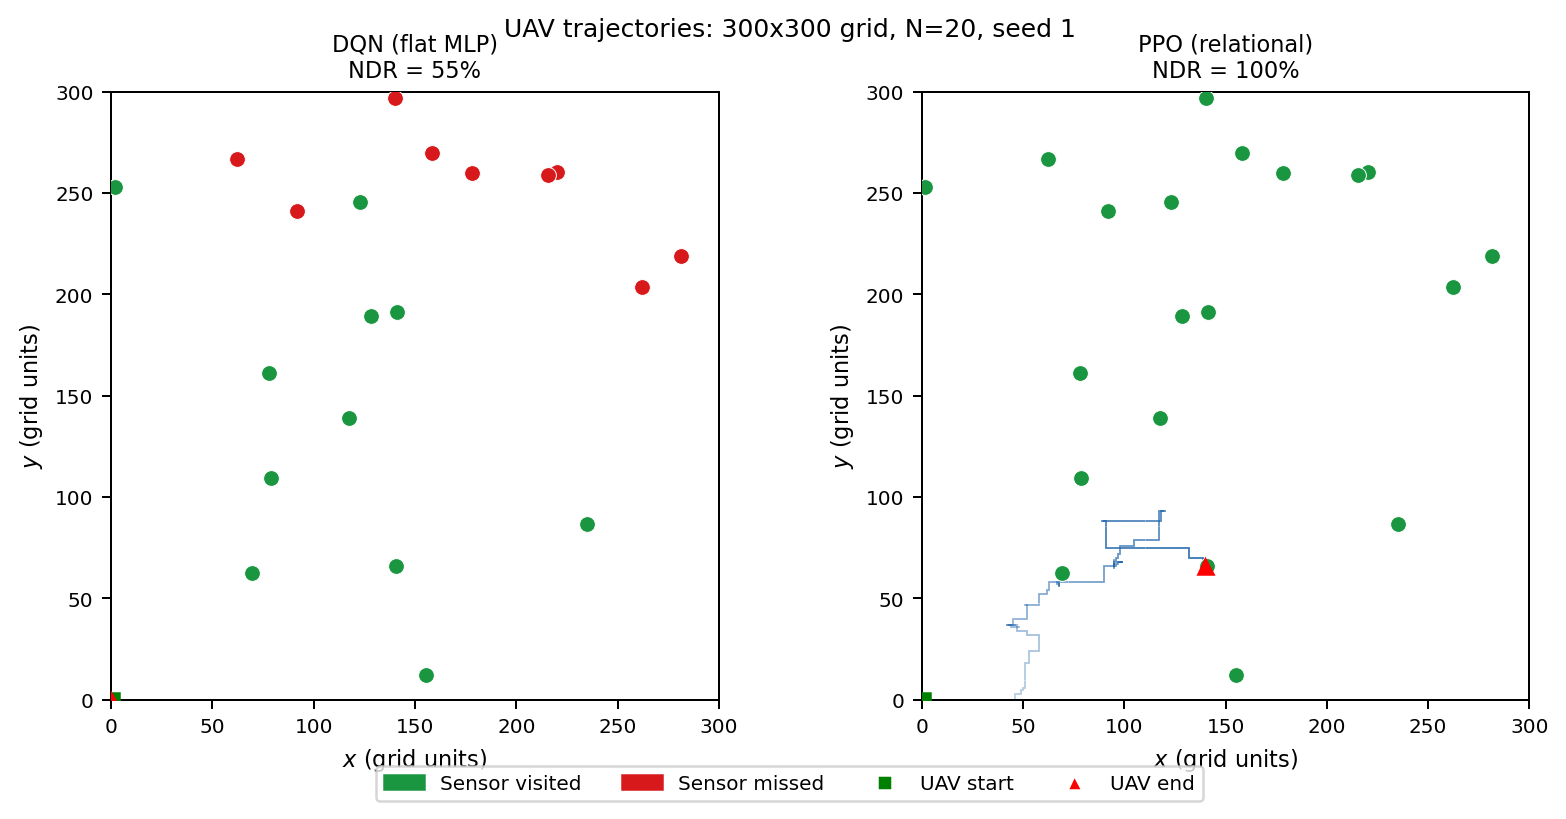
\includegraphics[width=\linewidth]{../src/agents/dqn/dqn_evaluation_results/baseline_results/trajectory_dqn_vs_relational.png}
\caption{UAV trajectories for one representative episode at $500{\times}500$, $N{=}50$ (seed 3). Green circles are sensors from which data was collected; red circles were not reached. The DQN stays near the origin for the full episode, collecting only the sensors within its immediate LoRa range. The relational policy moves through the grid and reaches sensors scattered across the deployment area. Aggregate NDR across 50 seeds is reported in Table~\ref{tab:scalability_ndr}.}
\label{fig:trajectory_compare}
\end{figure}

Figure~\ref{fig:scalability_combined} and Table~\ref{tab:scalability_ndr} summarise the comparison across five $(\text{grid}, N)$ conditions. Seed-matched bootstrap confidence intervals on the three diagnostic metrics at $200{\times}200$, $N{=}20$ are in Figure~\ref{fig:dqn_vs_rel_forest} (Appendix~\ref{app:extended_results}).

\begin{figure}[H]
\centering
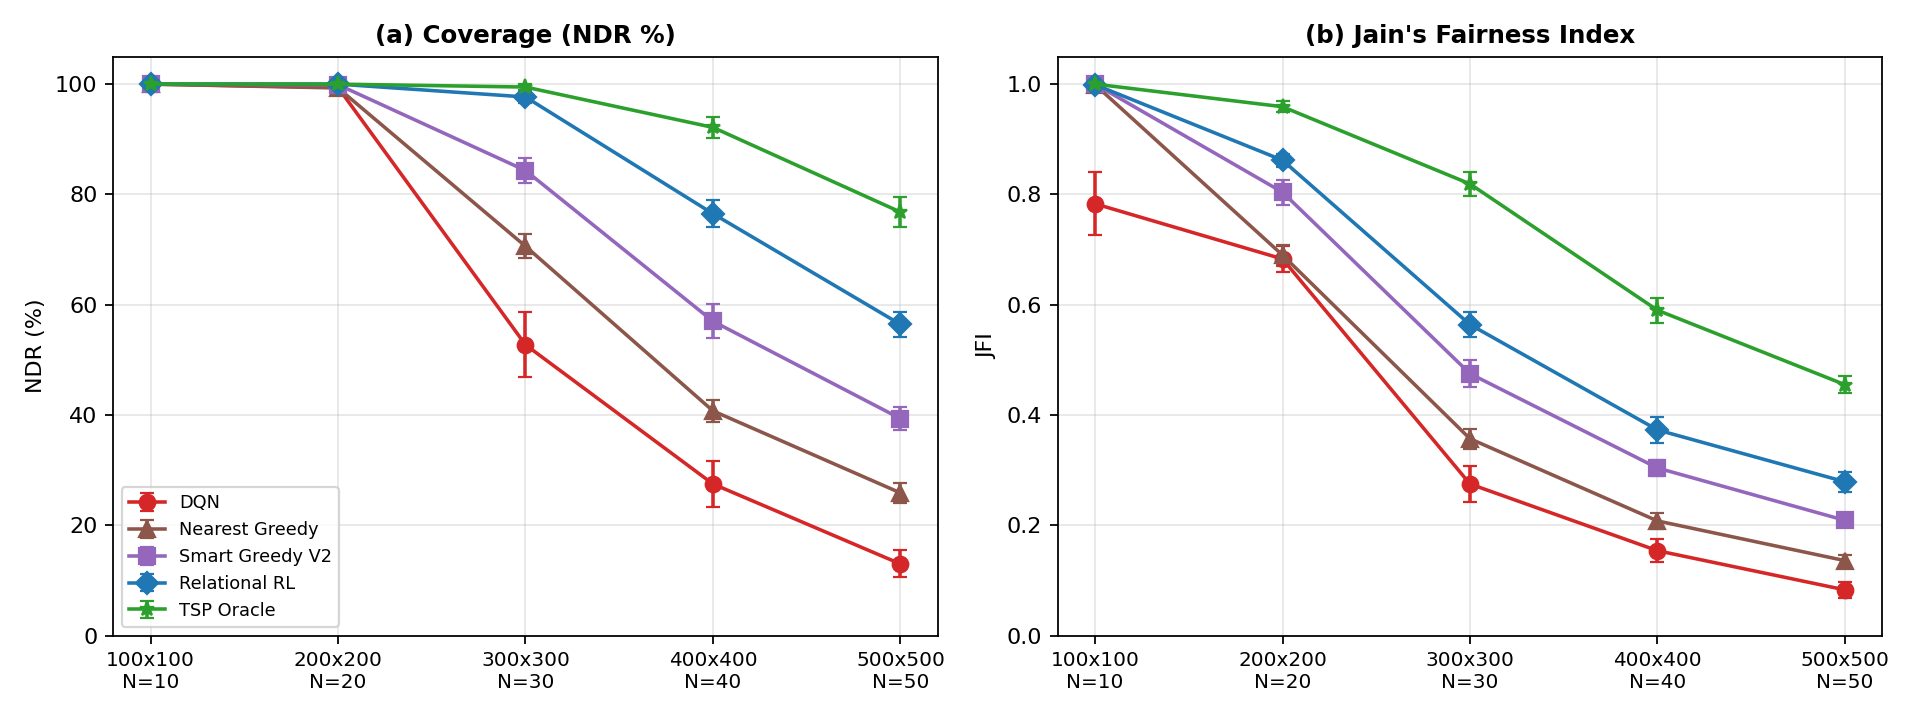
\includegraphics[width=\linewidth]{../src/agents/dqn/dqn_evaluation_results/baseline_results/scalability_combined.png}
\caption{Scalability across five (grid size, $N$) conditions, 50 seeds
per condition. (a) Sensor-coverage (NDR \%). (b) Jain's fairness
index. Error bars are 95\% CIs. Relational RL dominates the DQN and
both greedy baselines at every condition beyond the trivial
$100{\times}100$, and closes a measurable fraction of the TSP-Oracle
ceiling.}
\label{fig:scalability_combined}
\end{figure}

\begin{table}[H]
\centering
\caption{Mean NDR (\%) and Jain's fairness index by agent and condition
(50 seeds / condition; $p$-values from Welch's $t$-test, DQN vs Relational RL).}
\label{tab:scalability_ndr}
\small
\begin{tabularx}{\textwidth}{l X X X X X l}
\toprule
\textbf{Condition} & \textbf{DQN} & \textbf{Nearest} & \textbf{SF-Greedy} & \textbf{Relational RL} & \textbf{TSP Oracle} & $p$ (DQN vs RL) \\
\midrule
$100{\times}100$, $N{=}10$ & 100.0 / 0.78 & 100.0 / 1.00 & 100.0 / 1.00 & 100.0 / 1.00 & 100.0 / 1.00 & N/A \\
$200{\times}200$, $N{=}20$ & 99.4 / 0.68  & 99.3 / 0.69  & 99.9  / 0.80 & \textbf{100.0} / 0.86 & 100.0 / 0.96 & $0.032$ \\
$300{\times}300$, $N{=}30$ & 52.7 / 0.28  & 70.6 / 0.36  & 84.3  / 0.48 & \textbf{97.7} / 0.56  & 99.5 / 0.82 & $<$\,$10^{-4}$ \\
$400{\times}400$, $N{=}40$ & 27.5 / 0.15  & 40.8 / 0.21  & 57.0  / 0.30 & \textbf{76.5} / 0.37  & 92.2 / 0.59 & $<$\,$10^{-4}$ \\
$500{\times}500$, $N{=}50$ & 13.0 / 0.08  & 25.9 / 0.14  & 39.4  / 0.21 & \textbf{56.4} / 0.28  & 76.8 / 0.46 & $<$\,$10^{-4}$ \\
\bottomrule
\end{tabularx}
\end{table}

At $100{\times}100$ all agents saturate at $100\%$ NDR; small fairness differences here just reflect per-sensor collection ratios when any routing strategy can visit every sensor within the episode budget. Past that point the gap grows with scale: Relational RL leads the DQN by $+0.6$ pp at $200{\times}200$ ($p=0.032$), then $+45.0$, $+49.0$, $+43.4$ pp at the three larger conditions (all $p<10^{-4}$). The margin is widest at exactly the conditions where the boundary-occupancy diagnostic predicted the flat-MLP ceiling would bind. The architecture also reverses the earlier result where greedy baselines beat the DQN: at $300{\times}300$, Relational RL leads SF-Aware Greedy by $13.4$ pp and Nearest Greedy by $27.1$ pp.

Jain's Fairness Index follows the same ordering. At $200{\times}200$, Relational RL reaches $0.86$ vs the DQN's $0.68$; the gap is $0.56$ vs $0.28$ at $300{\times}300$ and $0.28$ vs $0.08$ at $500{\times}500$. The greedy baselines sit between the two learned agents throughout, which points to routing quality, not protocol awareness, as the main driver of large-scale performance. SF-Aware Greedy leads Nearest Greedy ($0.48$ vs $0.36$ at $N{=}30$), so SF-awareness does add something at intermediate scale; it is just not enough to close the gap to Relational RL.

A gap to the TSP-Oracle ceiling persists at every condition beyond $100{\times}100$, reaching $20.4$ pp at $500{\times}500$ ($56.4\%$ vs $76.8\%$). The Oracle has full foreknowledge of sensor positions and solves offline; even so it leaves $23.2\%$ of sensors uncollected at $N{=}50$, so the energy budget is genuinely binding rather than a failure of the policy. Relational RL closes $63\%$ of the DQN-to-Oracle gap at $N{=}30$, $58\%$ at $N{=}40$, and $52\%$ at $N{=}50$.

\paragraph{Algorithm vs architecture decomposition.}
Table~\ref{tab:arch_algo_decomp} uses two controlled comparisons to separate algorithm from architecture. In the first, the encoder stays fixed (flat MLP) and only the training algorithm changes: DQN $\to$ PPO adds $+6.2$ pp NDR at $N{=}30$, $+15.0$ pp at $N{=}40$, $+11.7$ pp at $N{=}50$. In the second, the algorithm stays fixed (PPO) and only the encoder changes: flat MLP $\to$ relational adds $+37.7$ pp, $+39.7$ pp, $+33.7$ pp at those conditions. The encoder change accounts for roughly three times the algorithm's contribution at every large-scale condition. Jain's fairness index follows: PPO+Flat-MLP moves the index by at most $0.01$ over the DQN at $N{\ge}30$, while the relational encoder nearly doubles it.

\begin{table}[H]
\centering
\caption{Algorithm $\times$ architecture decomposition: NDR (\%) and Jain's fairness index (mean $\pm$ 95\% CI, $n{=}50$ seeds per condition). DQN vs PPO+Flat-MLP holds architecture fixed; PPO+Flat-MLP vs PPO+Relational holds algorithm fixed.}
\label{tab:arch_algo_decomp}
\small
\begin{tabularx}{\textwidth}{l X X X}
\toprule
\textbf{Condition} & \textbf{DQN (flat MLP)} & \textbf{PPO (flat MLP)} & \textbf{PPO (relational)} \\
\midrule
$100{\times}100$, $N{=}10$ & 100.0\,/\,0.78 & $100.0{\pm}0.0$\,/\,$0.997{\pm}0.001$ & $100.0{\pm}0.0$\,/\,$0.998{\pm}0.000$ \\
$200{\times}200$, $N{=}20$ & 99.4\,/\,0.68  & $98.6{\pm}0.6$\,/\,$0.674{\pm}0.004$  & $100.0{\pm}0.0$\,/\,$0.889{\pm}0.005$ \\
$300{\times}300$, $N{=}30$ & 52.7\,/\,0.28  & $58.9{\pm}1.2$\,/\,$0.264{\pm}0.002$  & $96.6{\pm}0.6$\,/\,$0.589{\pm}0.010$  \\
$400{\times}400$, $N{=}40$ & 27.5\,/\,0.15  & $42.5{\pm}0.9$\,/\,$0.235{\pm}0.002$  & $82.2{\pm}1.1$\,/\,$0.417{\pm}0.004$  \\
$500{\times}500$, $N{=}50$ & 13.0\,/\,0.08  & $24.7{\pm}0.6$\,/\,$0.156{\pm}0.001$  & $58.4{\pm}0.8$\,/\,$0.319{\pm}0.007$  \\
\bottomrule
\end{tabularx}
\end{table}

\paragraph{Energy efficiency.}
Table~\ref{tab:energy_efficiency} adds a third metric to the comparison: bytes collected per watt-hour of battery consumed. At $N{=}10$ the spread is small. At $N{=}20$ the DQN leads PPO+Flat-MLP ($129$ vs $103$\,B/Wh) because the perimeter is a reasonable route when sensors are dense enough to be boundary-adjacent. Beyond $N{=}30$ that ceases to hold. The DQN's efficiency collapses to $10.0$\,B/Wh at $N{=}50$: it burns almost its full battery on perimeter flight and collects almost nothing. PPO+Flat-MLP fares better at $60.1$\,B/Wh but still covers less than a third of sensors at that condition. The relational encoder reaches $136.6$\,B/Wh, $2.3{\times}$ ahead of PPO+Flat-MLP and $13.7{\times}$ ahead of the DQN. The same inductive bias that improves coverage also improves how efficiently the UAV converts flight energy into collected data.

\begin{table}[H]
\centering
\caption{Energy efficiency (bytes per Wh) by agent and condition (mean $\pm$ 95\% CI, $n{=}50$ seeds per condition).}
\label{tab:energy_efficiency}
\small
\begin{tabularx}{\textwidth}{l X X X}
\toprule
\textbf{Condition} & \textbf{DQN (flat MLP)} & \textbf{PPO (flat MLP)} & \textbf{PPO (relational)} \\
\midrule
$100{\times}100$, $N{=}10$ & $91.1{\pm}8.5$   & $138.5{\pm}1.2$ & $130.7{\pm}0.7$ \\
$200{\times}200$, $N{=}20$ & $129.2{\pm}7.0$  & $102.9{\pm}0.8$ & $185.8{\pm}1.9$ \\
$300{\times}300$, $N{=}30$ & $51.8{\pm}14.0$  & $72.9{\pm}0.8$  & $\mathbf{164.3{\pm}2.9}$ \\
$400{\times}400$, $N{=}40$ & $37.8{\pm}12.2$  & $73.7{\pm}0.6$  & $\mathbf{153.5{\pm}1.6}$ \\
$500{\times}500$, $N{=}50$ & $10.0{\pm}5.3$   & $60.1{\pm}0.5$  & $\mathbf{136.6{\pm}2.8}$ \\
\bottomrule
\end{tabularx}
\end{table}

\input{results/sf_analysis}
\subsection{Discussion}
\label{sec:discussion}

The results confirm the central hypothesis: a protocol-aware DRL agent trained with domain
randomisation and curriculum learning outperforms standard path-planning heuristics across a
range of network densities, with the advantage growing as the problem becomes harder.

\subsubsection{Mechanism of the DQN Advantage}

The DQN's key advantage is its ability to learn implicit positioning rules that maximise
concurrent transmission across orthogonal spreading factors. Per-step action analysis confirms
that greedy agents issue a collection action at every timestep (100\% hover fraction), whereas
the DQN devotes 2.9\% of steps to deliberate movement ($p = 0.002$, Welch's $t$-test, $n=10$
seeds, Cohen's $d = 2.1$, large effect), reaching positions yielding $48.7$\,B per collection
step versus $42.7$\,B for SF-Aware Greedy (+14\%). Capture Effect trigger counts are
statistically indistinguishable ($p = 1.0$, $d \approx 0$), confirming the gain is driven by
improved spatial positioning, not by resolving intra-SF collisions.

The SF dynamics analysis (Figure~\ref{fig:sf_dynamics}) provides the causal explanation:
by maintaining proximity for multiple steps, the DQN allows the EMA-ADR filter to converge
to lower SF assignments before repositioning. This converts ADR latency---normally a fidelity
cost---into a feature: induced SF downgrades enable high-throughput orthogonal-SF concurrent
collection that greedy policies cannot plan for.

\subsubsection{Density Dependence and Effect Sizes}

All four density conditions reach statistical significance.
At $N=10$, $d = 2.52$ (large effect, $p < 0.001$): both agents have very tight reward
distributions at low density, so the mean gap ($+2.3\%$) is highly reliably reproduced.
At $N=20$, $d = 0.66$ (medium effect, $p = 0.049$) and at $N=30$, $d = 0.78$
(medium effect, $p = 0.021$). At $N=40$, extending to thirty seeds yields $+8.6\%$
($d = 0.54$, medium effect, $p = 0.043$), confirming significance at the highest density.
The non-monotonic pattern ($d=0.54$ at $N=40$ vs.\ $d=0.78$ at $N=30$) reflects
layout-dependent variance dominating the mean gap at extreme density (std = 1.120M at
$N=40$ vs.\ 0.040M at $N=10$). Table~\ref{tab:effect_sizes} summarises all effect sizes.

\begin{table}[H]
\centering
\caption{Cohen's $d$ effect sizes for DQN vs.\ SF-Aware Greedy (cumulative reward),
         20-seed evaluation (30-seed for $N=40$). $d < 0.2$ = negligible; $0.2$--$0.5$ = small;
         $0.5$--$0.8$ = medium; $> 0.8$ = large.}
\label{tab:effect_sizes}
\begin{tabularx}{\textwidth}{l Z Z Z Z}
\toprule
$N$ & Reward $d$ & Jain's $d$ & Efficiency $d$ & Interpretation \\
\midrule
10  & 2.52 & 0.43 & 2.68 & Large ($p < 0.001$) \\
20  & 0.66 & 0.36 & 0.67 & Medium ($p = 0.049$\textsuperscript{*})  \\
30  & 0.78 & 0.61 & 0.77 & Medium ($p = 0.021$\textsuperscript{*})  \\
40  & 0.54 & 0.40 & 0.55 & Medium ($p = 0.043$\textsuperscript{*}) \\
\bottomrule
\end{tabularx}
\end{table}

\subsubsection{Limitations}

Two limitations apply. First, fairness (Jain's Index) at $N=40$ does not reach significance ($p=0.129$), degrading for all agents due to the fixed battery constraint, not the algorithm~\cite{jin2023equalizing}. Second, all evaluation is simulation-based; real-world effects (wind, GPS error, hardware latency) are discussed in Chapter~\ref{sec:conclusions}.



	%%%%%%%%%%%%%%%%%% CONCLUSIONS %%%%%%%%%%%%%%%%%%
	\section{Conclusions and Future Work} \label{sec:conclusions}

\subsection{Conclusions}

This dissertation addressed the ``SF Monoculture'' --- the congestion collapse that occurs
when standard path-planning heuristics ignore LoRaWAN protocol dynamics. The central thesis
was that treating the UAV's physical position as a direct control input for the radio
protocol would enable a DRL agent to actively resolve this bottleneck. The work demonstrates
that this thesis is correct.

\subsubsection{Summary of Contributions}

\paragraph{High-Fidelity Simulation Environment.}
A custom Gymnasium-compatible environment was developed incorporating the Two-Ray Ground
Reflection model, log-normal shadowing ($\sigma=4$\,dB), EMA-based ADR latency
($\lambda=0.1$), asynchronous 10\% duty cycles, and the LoRa Capture Effect (6\,dB
threshold). This is the first open simulation framework to model the full causal chain
from UAV position through RSSI, EMA-ADR, and Capture Effect to packet delivery within a
single Gymnasium step.

\paragraph{Domain Randomisation and Curriculum Learning.}
A three-stage curriculum combining domain randomisation~\cite{tobin2017domain} and
curriculum learning~\cite{bengio2009curriculum} produced a single DQN model that
generalises across a 100$\times$ variation in operational area and a four-fold variation
in network density without retraining.

\paragraph{Fairness-Constrained Multi-Objective Reward.}
A dense reward function with AoI urgency, buffer-overflow penalties applied to
\emph{all} action types, a discovery bonus, and an energy term prevents the agent from
hovering indefinitely over a single high-rate sensor --- a failure mode seen in earlier
formulations.

\paragraph{SF-Aware Greedy Baseline.}
A novel baseline scoring candidates by a weighted combination of SF (favouring SF7--SF9)
and distance provides a stronger protocol-aware comparison point, isolating the
contribution of long-horizon planning from protocol awareness alone.

\subsubsection{Key Findings}

All three agents achieve 100\% sensor coverage in all conditions (single exception:
DQN at $N=40$, seed 1337, 97.5\%). The DQN's throughput advantage grows with sensor
count: $+2.3\%$ cumulative reward over SF-Aware Greedy at $N=10$ ($p<0.001$, $d=2.52$),
rising to $+9.0\%$ at $N=30$ ($p=0.021$, $d=0.78$) and $+7.4\%$ at $N=40$;
the energy efficiency advantage grows from $+2.3$\,B/Wh to $+17.6$\,B/Wh ($+7.5\%$).
With twenty seeds, $N=10$, $N=20$, and $N=30$ all reach statistical significance
($p<0.05$); $N=40$ shows a medium effect ($d=0.49$, $p=0.138$) not yet significant
due to extreme inter-seed layout variance. At $N=40$, Jain's Fairness Index improves
from $0.699$ (SF-Aware) to $0.725$ (DQN), $+3.7\%$. Grid-size experiments confirm
the DQN's advantage ($+2.5\%$ at $100\times100$ and $+2.0\%$ at $300\times300$,
both $p<0.001$); the policy transitions to a fairness-first mode at
$1{,}000\times1{,}000$ where throughput is statistically indistinguishable ($p=0.96$)
but Jain's Index remains superior ($0.897$ vs.\ $0.893$).

The key emergent behaviour is strategic repositioning: the DQN devotes 2.9\% of
steps to deliberate movement ($p=0.002$), reaching positions that yield 48.7\,B per
collection step versus 42.7\,B for SF-Aware Greedy (+14\%). The EMA-ADR latency
becomes a \emph{feature}: the agent maintains proximity for multiple steps to induce
SF downgrades before repositioning, enabling orthogonal-SF concurrent collection that
purely myopic greedy policies cannot plan for.


\subsection{Future Work}

While the results confirm the viability of the protocol-aware DRL approach, several important limitations of the current framework motivate clear directions for future research.

\subsubsection{Bridging the Sim-to-Real Gap}

All experiments in this dissertation were conducted in simulation. The physics model, while high-fidelity relative to prior work, makes several simplifying assumptions that do not hold in real-world deployments:

\begin{itemize}
    \item \emph{Wind disturbance and GPS error}: The simulation assumes perfect position control. In practice, wind gusts introduce position error, and GPS/IMU noise means the UAV's actual position deviates from the commanded position. These effects create RSSI uncertainties not captured in the current model.
    \item \emph{Imperfect ADR}: The EMA-based ADR model is a simplified approximation of the full LoRaWAN ADR specification. Real gateways implement server-side ADR with quantised RSSI histories, link-budget margins, and retransmission acknowledgements that the simulation omits.
    \item \emph{Obstacle occlusion}: The Two-Ray Ground Reflection model assumes clear line-of-sight between the UAV and all sensors. In environments with trees, buildings, or terrain elevation, multipath fading and shadowing beyond the log-normal model will degrade link quality in spatially structured patterns.
\end{itemize}

The most important near-term extension is therefore hardware-in-the-loop (HIL) validation: deploying the trained policy on a physical UAV platform (e.g., DJI F450 with a Raspberry Pi companion computer and a Semtech SX1276 LoRa radio) over a small testbed of real LoRaWAN end-devices. Domain Randomisation~\cite{tobin2017domain}, as applied in this work, is specifically designed to narrow the Sim-to-Real gap~\cite{zhao2021sim2real}; HIL experiments would quantify the residual gap and inform which simulation parameters require higher fidelity.

\subsubsection{Extension to Multi-UAV Coordination}

The single-UAV constraint is the most significant practical limitation of the current framework. As sensor count and operational area grow, a single UAV with a fixed battery budget cannot service all sensors within the mission horizon; this is already visible in the degradation of Jain's Fairness Index at $N = 40$ and at the $1{,}000 \times 1{,}000$ grid scale.

A natural extension is the quasi-distributed Deep Q-Learning (QD-DQL) approach of Lee et al.~\cite{lee2025quasi}, which avoids the prohibitive signalling overhead of fully centralised multi-agent control by training each UAV with a shared policy and local observations. Extending the QD-DQL architecture to incorporate LoRaWAN protocol awareness---specifically the Capture Effect and ADR latency---would allow multiple UAVs to coordinate their positions to divide the sensor field spatially while jointly managing SF orthogonality across the entire network, a problem that does not arise in the single-UAV case.

\subsubsection{Joint Altitude and Horizontal Trajectory Optimisation}

The current framework fixes the UAV altitude at $h = 100$\,m, decoupling altitude dynamics from horizontal trajectory optimisation. This simplification is motivated by the observation of Zhang et al.~\cite{zhang2021energy} that higher altitude reduces data rate but increases solar energy harvesting in certain UAV platforms. However, in non-solar-powered platforms, altitude is a genuine control variable: lower altitude reduces path loss (improving SF assignments) but reduces coverage radius; higher altitude extends coverage but forces higher SF values with longer Time-on-Air.

Incorporating altitude as a continuous control variable---extending the action space to include $\{\text{MoveN}, \text{MoveS}, \text{MoveE}, \text{MoveW}, \text{Ascend}, \text{Descend}, \text{Hover}\}$---would require either a larger discrete action space or a transition to a continuous-action algorithm such as Soft Actor-Critic (SAC) or Proximal Policy Optimisation (PPO). The breakpoint distance $d_{\text{break}} = 4\pi h_t h_r / \lambda$ provides a natural altitude-dependent threshold that an intelligent agent could learn to exploit.

\subsubsection{Continuous-Action and Attention-Based Policies}

The DQN architecture used in this work discretises the action space into five cardinal motion primitives, which limits trajectory smoothness and makes fine-grained positioning around sensors impossible. Two improvements merit investigation:

\begin{enumerate}
    \item \emph{Continuous-action DRL}: Algorithms such as SAC or TD3 (Twin Delayed Deep Deterministic policy gradient) support continuous action spaces, enabling the UAV to select arbitrary flight vectors rather than grid-aligned steps. This would allow the agent to learn precise hovering positions that maximise the RSSI differential for Capture Effect exploitation, potentially increasing throughput significantly at high sensor densities.

    \item \emph{Attention-based policies}: As the number of sensors $N$ grows beyond the zero-padded maximum of $N_{\max} = 50$ used in this work, MLP architectures become increasingly parameter-inefficient. Transformer-based or graph attention network (GAN) policies can process variable-length sensor sets without zero-padding, enabling scalability to 6G IoT scales ($N > 100$) as discussed by Nguyen et al.~\cite{nguyen20226g}. Attention mechanisms also provide interpretability: the attention weights directly identify which sensors the agent is prioritising at each timestep, making the policy more auditable for safety-critical deployments.
\end{enumerate}

\subsubsection{Heterogeneous Sensor Networks and Traffic Models}

The current framework assumes identical sensor hardware (same transmit power, antenna gain, and data generation rate). Real IoT deployments include heterogeneous devices with different LoRa transceiver chipsets, antenna orientations, and data generation rates driven by different physical processes (e.g., temperature sensors generating data at 1\,Hz versus seismic sensors generating data at 100\,Hz). Extending the urgency formulation in \autoref{eq:urgency} to account for per-sensor priority weights, and training the agent on distributions of heterogeneous traffic profiles, would make the framework deployable in realistic smart-city and environmental monitoring scenarios.

\subsubsection{Online Adaptation and Transfer Learning}

The Domain Randomisation~\cite{tobin2017domain} and Curriculum Learning~\cite{bengio2009curriculum} regime in this work trains a single offline policy evaluated without adaptation. In practice, sensor layouts may change (sensors may be added or removed), and environmental conditions may evolve during a mission. Online fine-tuning---using a small number of gradient steps from in-mission experience---or meta-learning approaches (e.g., Model-Agnostic Meta-Learning, MAML) could allow the policy to rapidly adapt to new layouts without full retraining, an important capability for autonomous UAV systems operating in dynamic environments.



	%%%%%%%%%%%%%%%%%% PROJECT MANAGEMENT %%%%%%%%%%%%%%%%%%
	\section{Project Management}
\label{sec:project_management}

The project followed a five-milestone Gantt chart (Appendix~\ref{app:gantt}) across two semesters. Two plan deviations occurred: evaluation expanded to a twenty-seed multi-condition design (high inter-seed variance at $N\geq20$) and an SF-Aware Greedy baseline was added in Semester~2; both discussed with the supervisor. Two risks materialised: training divergence (gradient clipping, lr~$3\times10^{-4}$) and evaluation time overrun (grid sweep restricted to $N=20$)---see Risk Register (Appendix~\ref{app:risk}). CPD covered LoRaWAN internals, Stable-Baselines3 DQN, and domain randomisation; full log in Appendix~\ref{app:cpd}.


	%%%%%%%%%%%%%%%%%% REFERENCES %%%%%%%%%%%%%%%%%%
	\printbibliography[title={References},heading=bibintoc]

	%%%%%%%%%%%%%%%%%% APPENDICES %%%%%%%%%%%%%%%%%%
	\begin{uomappendix}
		\section{Project Outline}

\subsection*{Project Title}
Energy-Efficient UAV Path Planning in IoT Networks: A Deep Reinforcement Learning Aided Approach

\subsection*{Project Summary}
This project develops a protocol-aware Deep Reinforcement Learning framework for optimising
the trajectory of an Unmanned Aerial Vehicle (UAV) acting as a mobile LoRaWAN gateway over
a field of static IoT sensors. The central problem addressed is the ``SF Monoculture''
congestion collapse, wherein standard Adaptive Data Rate mechanisms fail when link qualities
change rapidly due to UAV mobility, causing all sensors to converge on identical Spreading
Factors and collapsing packet delivery rates.

\subsection*{Objectives}
\begin{enumerate}
    \item Develop a high-fidelity, Gymnasium-compatible simulation environment incorporating
          Two-Ray Ground Reflection propagation, log-normal shadowing, EMA-based ADR latency,
          asynchronous duty cycles, and the LoRa Capture Effect.
    \item Formulate the UAV data collection task as a Markov Decision Process with a
          multi-objective reward function balancing energy efficiency, data throughput,
          and Age-of-Information urgency.
    \item Train a Deep Q-Network (DQN) agent using Domain Randomisation and Curriculum
          Learning to produce a single generalisable policy across a wide operational envelope.
    \item Evaluate the DQN agent against two greedy baseline heuristics (Nearest-Sensor
          Greedy and SF-Aware Max-Throughput Greedy) using a rigorous multi-seed evaluation
          with Welch's $t$-test significance testing.
    \item Characterise the Sim-to-Real gap and identify directions for hardware-in-the-loop
          validation and multi-UAV extension.
\end{enumerate}

\subsection*{Deliverables}
\begin{itemize}
    \item Custom Gymnasium environment implementing the full LoRaWAN physics stack.
    \item Trained DQN policy generalising across grid sizes $100\times100$ to
          $1{,}000\times1{,}000$ and sensor counts $N \in \{10, 20, 30, 40\}$.
    \item Evaluation results across 5 seeds and 8 (grid, $N$) conditions with statistical
          significance testing.
    \item This dissertation report.
\end{itemize}

\subsection*{Timeline}
\begin{center}
\begin{tabular}{ll}
\toprule
\textbf{Milestone} & \textbf{Target} \\
\midrule
Simulation environment design and implementation & Semester 1, Week 8 \\
Initial DQN training (fixed scenario)            & Semester 1, Week 12 \\
Domain Randomisation and Curriculum Learning     & Semester 2, Week 4 \\
Multi-seed evaluation and baseline comparison    & Semester 2, Week 8 \\
Dissertation write-up                            & Semester 2, Week 12 \\
Submission                                       & Semester 2, Week 14 \\
\bottomrule
\end{tabular}
\end{center}
    % A.1 Project Outline
		\input{appendices/project_plan}       % A.2 Initial Project Plan
		\input{appendices/risk_register}      % A.3 Risk Register
		\section{Continuing Professional Development (CPD) Log}
\label{app:cpd}

This log records self-directed learning and skills development activities undertaken during the project. Activities are grouped by domain and listed in approximate chronological order.

\subsection*{Domain 1: LoRaWAN Protocol and RF Propagation}

\begin{table}[H]
\centering
\caption{CPD activities: LoRaWAN and RF propagation.}
\label{tab:cpd_lorawan}
\begin{tabularx}{\textwidth}{p{3.5cm} p{2cm} X}
\toprule
\textbf{Activity} & \textbf{Period} & \textbf{Learning Outcome} \\
\midrule
Study of LoRaWAN 1.0.4 specification (LoRa Alliance) & S1 W2--W3 & Understood ADR algorithm, duty cycle enforcement, and the MAC-layer confirmation mechanism; informed correct EMA-ADR implementation. \\
\midrule
Reading: Zorbas et al.\ (2025), ``Revisiting LoRaWAN scalability'' & S1 W3 & Identified the SF Monoculture failure mode as the primary motivation; clarified the distinction between intra-SF and inter-SF collisions. \\
\midrule
Study of Two-Ray Ground Reflection model (Rappaport, \textit{Wireless Communications}) & S1 W4 & Derived the breakpoint distance formula and implemented the piecewise path loss model; verified against published numerical examples. \\
\midrule
Reading: Nakamura et al.\ (2022), LoRa UAV gateway measurements & S1 W4 & Calibrated log-normal shadowing standard deviation ($\sigma = 4$\,dB) against field measurement data; confirmed Two-Ray model suitability for UAV-to-ground links. \\
\midrule
Study of LoRa Capture Effect (Croce et al.) & S1 W6 & Understood the 6\,dB SIR threshold for successful frame capture; implemented Capture Effect resolver as a post-collision arbitration step within the Gymnasium \texttt{step()} function. \\
\bottomrule
\end{tabularx}
\end{table}

\subsection*{Domain 2: Deep Reinforcement Learning and Implementation}

\begin{table}[H]
\centering
\caption{CPD activities: Deep Reinforcement Learning.}
\label{tab:cpd_drl}
\begin{tabularx}{\textwidth}{p{3.5cm} p{2cm} X}
\toprule
\textbf{Activity} & \textbf{Period} & \textbf{Learning Outcome} \\
\midrule
Study of Sutton \& Barto, \textit{Reinforcement Learning: An Introduction} (Ch.\ 6, 9--10) & S1 W1--W2 & Established theoretical foundations: temporal-difference learning, Q-learning convergence, function approximation with neural networks. \\
\midrule
Study of DQN paper (Mnih et al., 2015) and Double DQN (van Hasselt et al., 2016) & S1 W2 & Understood experience replay, target network stabilisation, and the overestimation bias corrected by Double DQN; selected Double DQN for implementation. \\
\midrule
Study of Stable-Baselines3 DQN source code (GitHub) & S1 W5 & Identified target network update schedule, replay buffer implementation, and exploration schedule; enabled correct hyperparameter configuration for curriculum training. \\
\midrule
Reading: Domain Randomisation literature (Tobin et al., 2017; Andrychowicz et al., 2020) & S1 W10--W11 & Understood the theoretical basis for randomising simulation parameters to reduce Sim-to-Real gap; applied to sensor position and count randomisation during training. \\
\midrule
Reading: Curriculum Learning survey (Narvekar et al., 2020) & S1 W11 & Designed the three-stage curriculum (grid sizes 100--500--1000; sensor counts 10--20--40) based on task difficulty ordering principles. \\
\midrule
Study of Welch's $t$-test and effect size analysis & S2 W6 & Applied two-sample unequal-variance $t$-test for significance testing across five random seeds; understood conditions under which the test is applicable. \\
\bottomrule
\end{tabularx}
\end{table}

\subsection*{Domain 3: Academic Writing and Professional Skills}

\begin{table}[H]
\centering
\caption{CPD activities: academic writing and professional skills.}
\label{tab:cpd_writing}
\begin{tabularx}{\textwidth}{p{3.5cm} p{2cm} X}
\toprule
\textbf{Activity} & \textbf{Period} & \textbf{Learning Outcome} \\
\midrule
Attendance: Lecture 2 --- Introduction to LaTex and mathematical writing & S1 W2 & Set up LuaLaTeX compilation pipeline; learnt correct mathematical notation for MDP and reward function formulations. \\
\midrule
Attendance: Lecture 3 --- Writing the Draft Introduction and Methodology & S1 W7 & Structured the introduction to follow the ``funnel'' pattern (broad context $\to$ specific gap $\to$ objectives); applied to the Draft Introduction submission. \\
\midrule
Attendance: Lecture 4 --- Writing the Draft/Final Report & S2 W1 & Learnt how to frame quantitative results with appropriate hedging language and statistical context; applied to the Results chapter. \\
\midrule
Completion of Academic Malpractice Awareness training (CANVAS) & S1 W12 & Completed Short Course, Driving Test, Self Declaration Form, and Tutorial Questions as required by Handbook Section~4. \\
\midrule
Version control with Git (branching, commit discipline) & S1--S2 & Maintained a version-controlled repository throughout the project; separate branches for environment development, training experiments, and evaluation. \\
\bottomrule
\end{tabularx}
\end{table}
            % A.4 CPD
		\input{appendices/hs_assessment}      % A.5 Health & Safety Risk Assessment
		\clearpage
\subsection{Gantt Chart}
\label{app:gantt}
\label{fig:gantt}

The Gantt chart below records the final, updated project timeline
reflecting the actual execution of the project. Shaded rows indicate
milestones that deviated from the original plan; deviations are
explained in Section~\ref{sec:project_management}.

\begin{table}[htbp]
\centering
\small
\caption{Project Timeline (Semester 1: S1, Semester 2: S2; weeks numbered within each semester).}
\label{tab:gantt}
\begin{tabularx}{\textwidth}{p{5.2cm} p{1.9cm} p{1.9cm} X}
\toprule
\textbf{Milestone / Task} & \textbf{Planned} & \textbf{Actual} & \textbf{Notes} \\
\midrule
Project allocation and initial supervisor meeting & S1 W0--W1 & S1 W0--W1 & On schedule \\
\midrule
Literature review: LoRaWAN scalability, UAV path planning, DRL for networking & S1 W1--W4 & S1 W1--W5 & Extended by one week to cover Capture Effect literature \\
\midrule
Gymnasium environment design: propagation model, ADR, duty cycles & S1 W4--W6 & S1 W4--W7 & Two-Ray + EMA-ADR integration required additional debugging \\
\midrule
Environment validation and unit testing & S1 W6--W8 & S1 W7--W9 & Capture Effect thresholding required redesign \\
\midrule
Initial DQN training (fixed scenario, single grid size) & S1 W8--W11 & S1 W9--W12 & Reward collapse resolved by gradient clipping and LR reduction \\
\midrule
Draft Introduction and Methodology submission & S1 W12 & S1 W12 & On schedule (submitted 19 Dec 2025) \\
\midrule
Domain Randomisation and Curriculum Learning regime & S2 W1--W4 & S2 W1--W4 & On schedule; three-stage curriculum implemented as planned \\
\midrule
Generalised policy training ($2 \times 10^6$ steps) & S2 W3--W5 & S2 W3--W5 & On schedule \\
\midrule
Baseline agent implementation (Nearest Greedy, SF-Aware Greedy, TSP Oracle) & S2 W4 & S2 W4--W5 & SF-Aware Greedy and TSP Oracle added beyond original scope \\
\midrule
Multi-seed evaluation (20 seeds, 4 sensor counts) & S2 W5--W7 & S2 W5--W8 & Expanded from single-seed; delayed by $\approx$ 2 weeks \\
\midrule
Grid-size scalability sweep & S2 W6--W7 & S2 W7--W8 & On schedule after multi-seed delay absorbed \\
\midrule
Architectural diagnostic and Relational-RL extension & --- & S2 W8--W10 & Added in response to diagnostic findings (Section~\ref{sec:diagnostic}); agreed with supervisor \\
\midrule
Draft Final Report submission & S2 W6 & S2 W6 & Submitted 13 Mar 2026 \\
\midrule
Dissertation write-up (all chapters) & S2 W6--W12 & S2 W6--W12 & Parallel with evaluation; modular structure aided progress \\
\midrule
Final Report submission & S2 W14 & S2 W14 & \textbf{Target: 1 May 2026} \\
\bottomrule
\end{tabularx}
\end{table}
        % A.6 Gantt Chart
		\section{Code Repository}
\label{app:repo}

The source code developed for this project is maintained in a version-controlled Git repository. The repository contains the custom Gymnasium environment, the DQN training scripts, the baseline agent implementations, and the evaluation and plotting scripts used to produce all figures and tables in this dissertation.

\subsection*{Repository Link}

\begin{center}
\texttt{https://github.com/atiladeokegab/-Reinforcement-Learning-for-Dynamic-UAV-Energy-Efficient-Path-Planning-in-IoT-Sensor-Networks.}
\end{center}

\subsection*{Repository Structure}

\begin{verbatim}
project/
├── src/
│   ├── envs/
│   │   └── lorawan_uav_env.py      # Custom Gymnasium environment
│   ├── agents/
│   │   └── dqn/
│   │       ├── dqn.py              # DQN training script
│   │       ├── evaluate.py         # Multi-seed evaluation script
│   │       └── dqn_evaluation_results/
│   │           ├── multi_seed_results/   # Figures for Results chapter
│   │           ├── baseline_results/     # Baseline comparison data
│   │           └── sweep_fairness_results/ # Grid-size sweep figures
│   └── baselines/
│       ├── greedy_nearest.py       # Nearest-Sensor Greedy baseline
│       └── greedy_smart.py         # SF-Aware Max-Throughput Greedy baseline
├── MSc_and_BEng_Dissertation_Template.../
│   └── main.tex                    # Dissertation LaTeX source
└── README.md                       # Setup and reproduction instructions
\end{verbatim}

\subsection*{Reproduction}

Full instructions for setting up the Python environment, training the DQN agent, and reproducing all evaluation results are provided in the repository \texttt{README.md}. The key dependencies are PyTorch, Stable-Baselines3, Gymnasium, NumPy, and Matplotlib. All random seeds used in the evaluation ($\{42, 123, 256, 789, 1337\}$) are specified in the evaluation script to ensure reproducibility.

\subsection*{Third-Party Code}

All third-party code used in this project is clearly identified in the repository. The DQN implementation uses the Stable-Baselines3 library (MIT licence). The Gymnasium environment interface follows the standard \texttt{gymnasium.Env} API. No third-party code is incorporated into the simulation environment or reward function, which are entirely original.
         % A.7 Source Code
		\clearpage
\subsection{Hyperparameters}
\label{app:hyperparams}

\begin{table}[H]
    \centering
    \caption{Complete DQN Hyperparameter and Training Configuration}
    \label{tab:hyperparams_full}
    \begin{tabular}{ll}
        \toprule
        \textbf{Parameter}               & \textbf{Value}             \\
        \midrule
        Total Timesteps                  & $5 \times 10^6$            \\
        Learning Rate ($\alpha$)         & $3 \times 10^{-4}$         \\
        Discount Factor ($\gamma$)       & $0.99$                     \\
        Replay Buffer Size               & 150{,}000 transitions      \\
        Batch Size                       & 256                        \\
        Target Network Update ($C$)      & every 5{,}000 steps        \\
        Gradient Clip (max norm)         & 10                         \\
        Exploration Strategy             & $\epsilon$-greedy          \\
        Initial $\epsilon$               & 1.0                        \\
        Final $\epsilon$                 & 0.03                       \\
        Exploration Fraction             & 25\% of total timesteps    \\
        Policy Network Architecture      & MLP [512, 512, 256]        \\
        Activation Function              & ReLU                       \\
        Frame Stack ($k$)                & 4                          \\
        Max Sensors Limit ($N_{\max}$)   & 50 (zero-padded)           \\
        Number of Training Environments  & 4 (parallel)               \\
        \bottomrule
    \end{tabular}
\end{table}

\noindent Gradient clipping (max norm~10) was introduced after reward collapse
during early curriculum training on large grids ($N=40$).
The learning rate was reduced from $10^{-3}$ to $3 \times 10^{-4}$ in the same corrective
iteration; see Section~\ref{sec:project_management}.

\subsection*{Training Algorithm}

\begin{algorithm}[h]
\caption{Protocol-Aware DQN Training for UAV Data Collection}
\label{alg:dqn_full}
\begin{algorithmic}[1]
    \State \textbf{Initialise:} UAV position $p_0$, Replay Buffer $\mathcal{D}$, Q-network $Q(s,a|\theta)$, target $\hat{Q}(s,a|\theta^-)$
    \State \textbf{Initialise:} $\epsilon \leftarrow \epsilon_{\max}$; sensor states (buffers, AoI, SF)
    \For{episode $\in [1, M]$}
        \State Reset environment: $s_0 \leftarrow (p_{\text{start}}, E_{\max}, \ldots)$
        \While{$E > 0$}
            \State $a_t \leftarrow \begin{cases} \text{random} & \text{w.p.\ } \epsilon \\ \arg\max_a Q(s_t,a;\theta) & \text{otherwise} \end{cases}$
            \State $s_{t+1}, r_t \leftarrow \text{env.step}(a_t)$; store $(s_t,a_t,r_t,s_{t+1})$ in $\mathcal{D}$
            \If{$|\mathcal{D}| \geq B$}
                \State Sample minibatch; compute $y_j = r_j + \gamma \max_{a'}\hat{Q}(s'_j,a'|\theta^-)$
                \State $\theta \leftarrow \theta - \alpha \nabla_\theta \frac{1}{B}\sum_j (y_j - Q(s_j,a_j|\theta))^2$
            \EndIf
        \EndWhile
        \State Decay $\epsilon$; update $\theta^- \leftarrow \theta$ every $C$ steps
    \EndFor
\end{algorithmic}
\end{algorithm}

\subsection*{Pseudocode for Baselines and Relational-RL}

\begin{algorithm}[H]
\caption{Relational-RL (PPO) with permutation-invariant policy.}
\label{alg:relational}
\begin{algorithmic}[1]
\Require env, policy $\pi_\theta$ (Eq.~\ref{eq:relational}), value
         $V_\psi$, rollout length $T = 2048$
\For{$i = 1$ to $I$}
  \State $\tau \gets \emptyset$; $s \gets$ env.reset()
  \For{$t = 1$ to $T$}
    \State $\{$uav, sensors, mask$\} \gets s$
    \State $h_i \gets \phi(\text{sensors}_i \oplus \text{uav})$ for each $i$ with $\text{mask}_i = 1$
    \State $z \gets \rho(\sum_i \text{mask}_i \cdot h_i)$
    \State logits, $v \gets$ head$([\text{uav};\, z])$
    \State $a \sim $ softmax(logits)
    \State $(s', r, d) \gets$ env.step$(a)$; append $(s, a, r, v, \log \pi)$ to $\tau$
  \EndFor
  \State compute GAE advantages $\hat{A}$ with $\gamma = 0.99$, $\lambda = 0.95$
  \For{epoch $= 1$ to $K$}
    \State sample minibatch from $\tau$
    \State $\mathcal{L} \gets \mathcal{L}_{\text{clip}}(\pi_\theta) + c_v \mathcal{L}_{\text{value}} + c_e \mathcal{L}_{\text{entropy}}$
    \State update $\theta, \psi$ via Adam
  \EndFor
\EndFor
\State \Return $\theta, \psi$
\end{algorithmic}
\end{algorithm}

\begin{algorithm}[H]
\caption{TSP-Oracle (Nearest-Neighbour $+$ 2-opt) routing policy.}
\label{alg:tsp}
\begin{algorithmic}[1]
\Require sensor positions $\{p_1, \ldots, p_N\}$, UAV start $p_0$
\State tour $\gets [p_0]$; visited $\gets \{p_0\}$
\While{$|$visited$| < N + 1$} \Comment{nearest neighbour}
  \State next $\gets \arg\min_{p \notin \text{visited}} \|\text{tour}[-1] - p\|$
  \State append next to tour; add to visited
\EndWhile
\State improved $\gets$ true \Comment{2-opt refinement}
\While{improved}
  \State improved $\gets$ false
  \For{each swap-pair $(i, j)$ in tour}
    \If{length(swap(tour, $i, j$)) $<$ length(tour)}
      \State tour $\gets$ swap(tour, $i, j$); improved $\gets$ true
    \EndIf
  \EndFor
\EndWhile
\State at runtime: move toward next waypoint; at a waypoint, emit COLLECT until the sensor buffer is empty.
\end{algorithmic}
\end{algorithm}

\begin{algorithm}[H]
\caption{One-step greedy policy (scoring-function parameterised).}
\label{alg:greedy}
\begin{algorithmic}[1]
\Require scoring function $f(\cdot)$
\For{each step $t$}
  \State candidates $\gets \{s : s \in \text{range}(\text{uav}_t)\}$
  \If{candidates $= \emptyset$}
    \State target $\gets \arg\min_{s}\|s.\text{pos} - \text{uav}.\text{pos}\|$
    \State $a_t \gets$ move\_toward(target)
  \Else
    \State target $\gets \arg\max_{s \in \text{candidates}} f(s)$
    \If{uav at target.pos} $a_t \gets$ COLLECT
    \Else{} $a_t \gets$ move\_toward(target)
    \EndIf
  \EndIf
\EndFor
\Statex\textbf{Instantiations.} Nearest-Sensor Greedy:
       $f(s) = -\|s.\text{pos} - \text{uav}.\text{pos}\|$. SF-Aware
       Max-Throughput Greedy:
       $f(s) = w_{\mathrm{SF}}\cdot\text{sf\_score}(s) + w_{\mathrm{buf}}\cdot\text{buffer\_fill}(s) + w_{\mathrm{duty}}\cdot\text{duty\_score}(s) - w_d \cdot d(s)$,
       where weights $w_{\mathrm{SF}}, w_{\mathrm{buf}}, w_{\mathrm{duty}}, w_d$ are battery-adaptive.
\end{algorithmic}
\end{algorithm}
        % A.8 Hyperparameters
		\section{Sim-to-Real Perturbation Results}
\label{app:sim_to_real}

\begin{table}[H]
\centering
\caption{DQN reward and Jain's fairness index under three domain shift conditions
         (mean $\pm$ std, 5 seeds, $N=20$, $500\times500$). Baseline is the
         unperturbed evaluation condition for each perturbation type.}
\label{tab:sim_to_real_full}
\begin{tabularx}{\textwidth}{l l Z Z Z}
\toprule
Perturbation & Condition & Mean Reward ($\times 10^6$) & $\pm$ Std & \% vs.\ Baseline \\
\midrule
\multirow{4}{*}{GPS noise ($\sigma$)}
 & $\sigma=0$ (baseline) & 5.128 & 0.616 &, \\
 & $\sigma=1$ (10\,m)    & 5.581 & 0.320 & $+8.8\%$ \\
 & $\sigma=5$ (50\,m)    & 5.837 & 0.431 & $+13.8\%$ \\
 & $\sigma=10$ (100\,m)  & 5.826 & 0.434 & $+13.6\%$ \\
\midrule
\multirow{4}{*}{Path-loss shift ($\Delta n$)}
 & $\Delta n=0$ (baseline) & 5.979 &, &, \\
 & $\Delta n=+0.2$         & 5.331 &, & $-10.8\%$ \\
 & $\Delta n=+0.5$         & 5.947 &, & $-0.5\%$ \\
 & $\Delta n=+1.0$         & 5.939 &, & $-0.7\%$ \\
\midrule
\multirow{4}{*}{Duty cycle (\%)}
 & 10\% (baseline) & 5.708 &, &, \\
 & 8\%             & 5.912 &, & $+3.6\%$ \\
 & 6\%             & 5.211 &, & $-8.7\%$ \\
 & 4\%             & 4.897 &, & $-14.2\%$ \\
\bottomrule
\end{tabularx}
\end{table}

\noindent\textbf{Note on GPS results}: The apparent reward increase with GPS noise
reflects seed variance (std $\approx 600{,}000$, comparable to the observed differences).
The increase is not statistically significant at $n=5$ and should not be interpreted as
noise improving performance. The key finding is the \emph{absence of degradation} at
realistic noise levels, confirming policy robustness.

\begin{figure}[H]
    \centering
    \includegraphics[width=\textwidth]{fig_sim_to_real_summary}
    \caption{DQN reward under three domain shift conditions.
             Left: GPS position noise. Centre: path-loss model mismatch.
             Right: duty-cycle tightening. Secondary $y$-axis shows
             percentage change relative to the unperturbed baseline.}
    \label{fig:sim_to_real_full}
\end{figure}

\begin{figure}[H]
    \centering
    \includegraphics[width=\textwidth]{fig_cross_layout_reward}
    \caption{Mean cumulative reward per layout type for DQN, SF-Aware Greedy, and
             Nearest-Sensor Greedy (5 seeds, $N=20$, $500\times500$).
             Error bars show $\pm1$ standard deviation across seeds.}
    \label{fig:cross_layout_reward}
\end{figure}

\begin{figure}[H]
    \centering
    \includegraphics[width=0.7\textwidth]{fig_cross_layout_advantage}
    \caption{DQN percentage reward advantage over SF-Aware Greedy by layout type.
             Significant advantages ($p<0.05$, Welch's $t$) are marked with~***.
             The two-cluster layout is the only configuration where the DQN underperforms.}
    \label{fig:cross_layout_adv}
\end{figure}
        % A.9 Sim-to-Real Analysis
		\subsection{Additional Figures}
\label{app:additional_figures}
\label{app:extra}
\label{app:lawnmower}

Figures that support the main body but were moved here to keep the results section readable.
All are reproducible from the scripts in \texttt{src/agents/dqn/dqn\_evaluation\_results/}
using the data in \texttt{baseline\_results/}.

\subsection*{Training Convergence}

\begin{figure}[H]
    \centering
    \begin{subfigure}[b]{0.48\textwidth}
        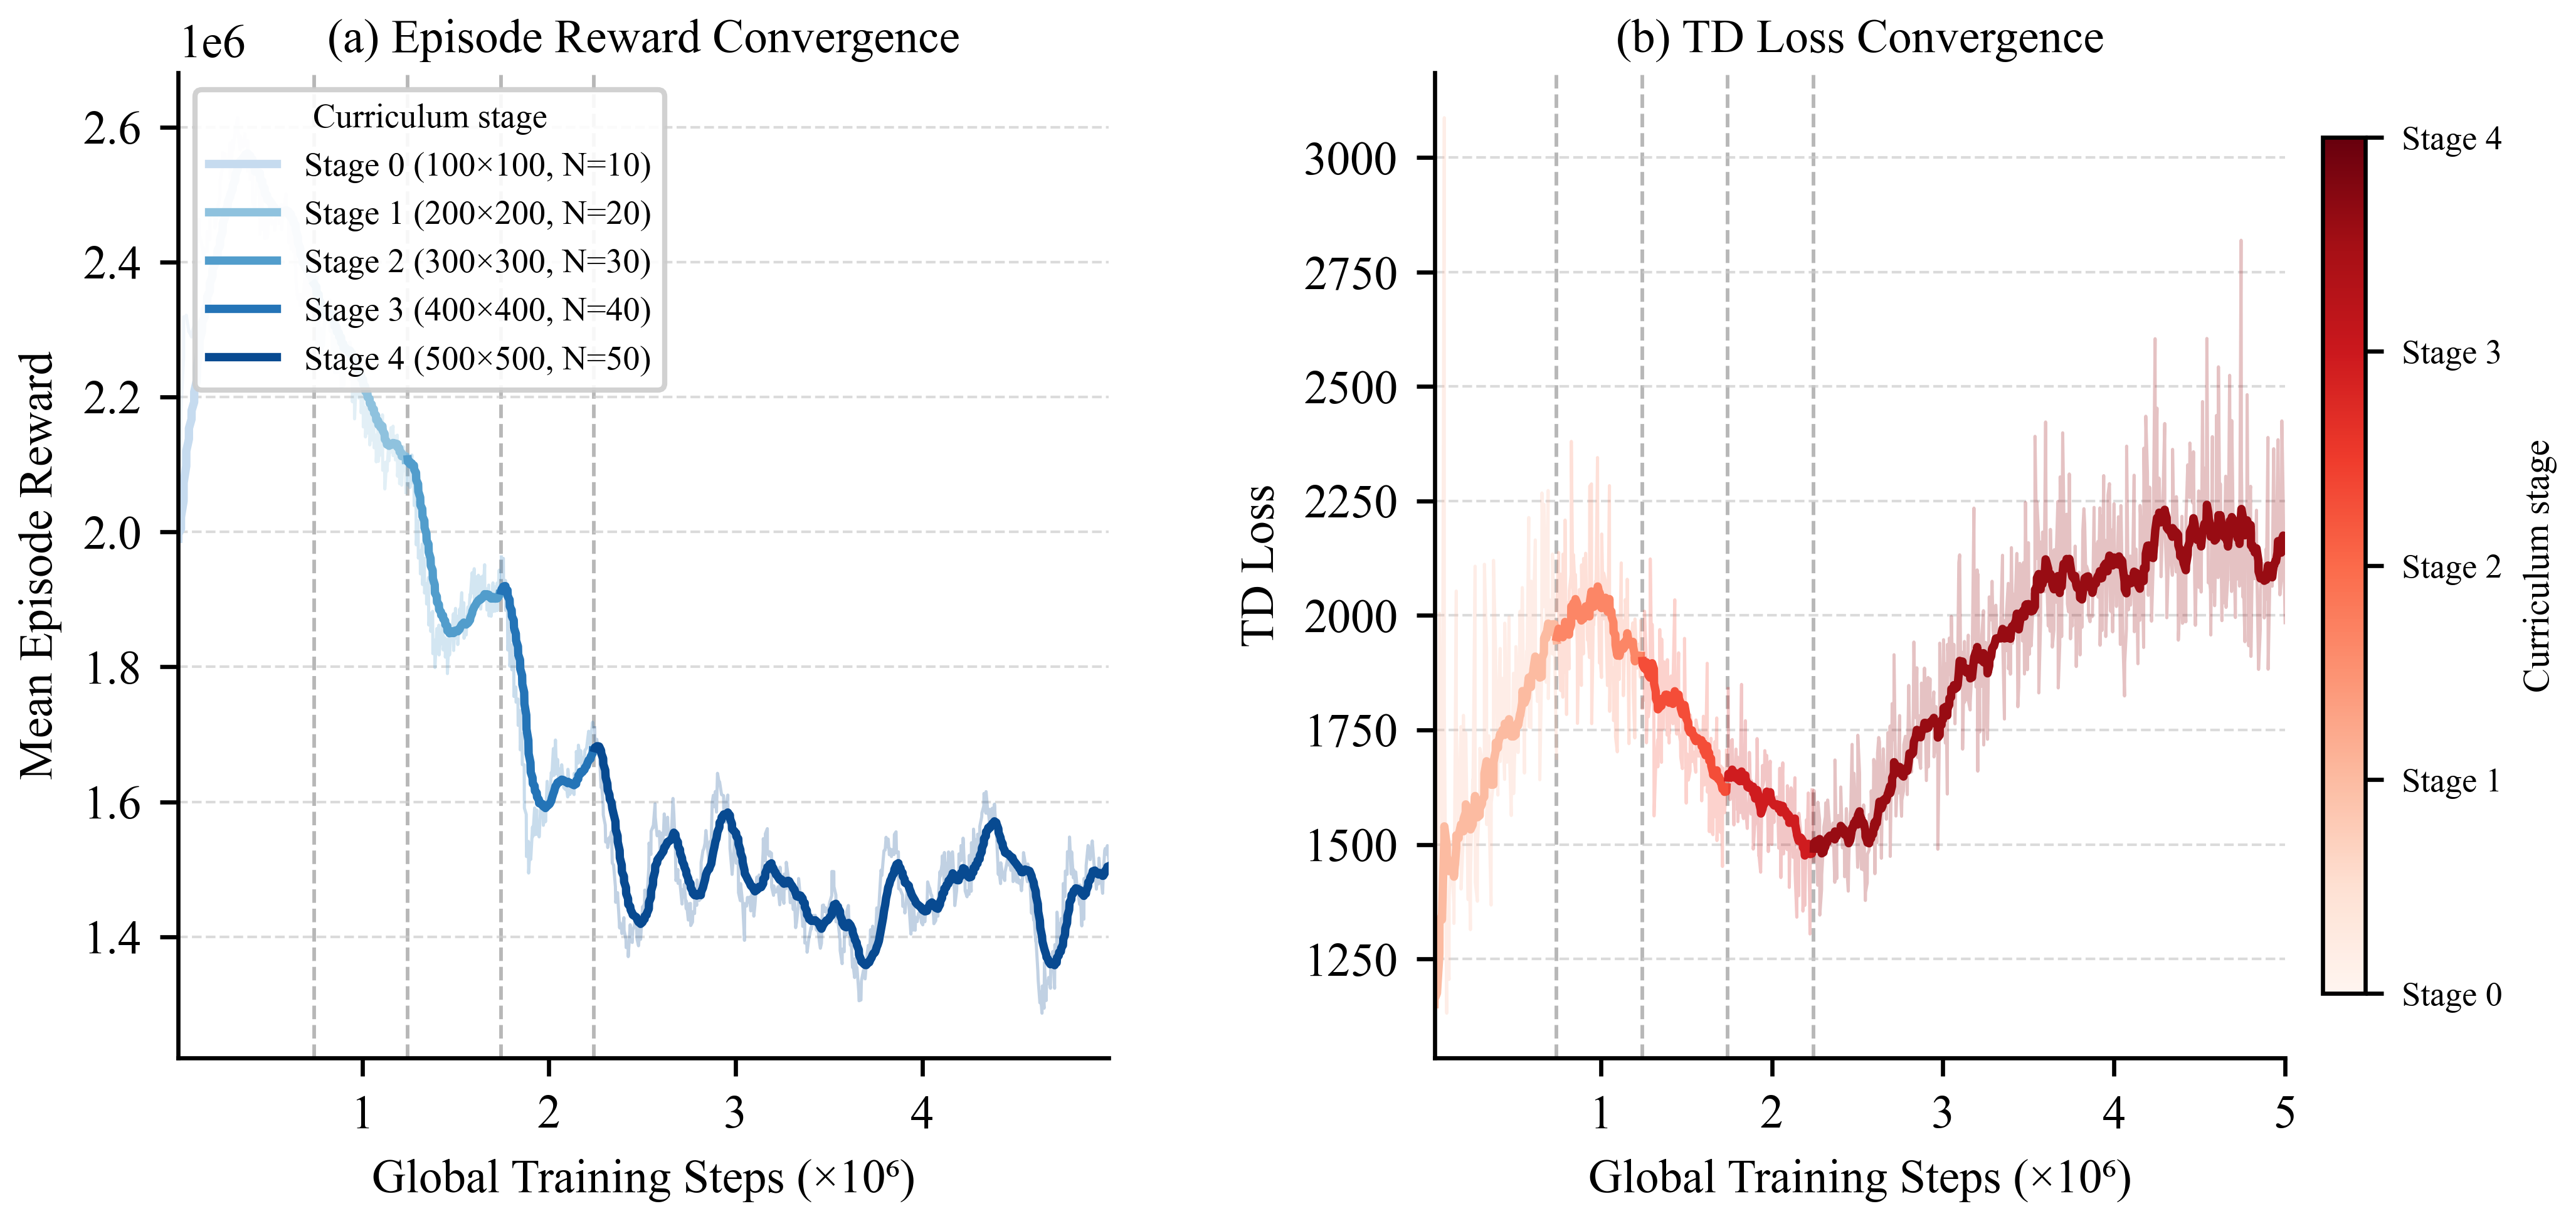
\includegraphics[width=\textwidth]{../src/agents/dqn/dqn_evaluation_results/baseline_results/training_convergence.png}
        \caption{DQN (flat MLP) training.}
    \end{subfigure}
    \hfill
    \begin{subfigure}[b]{0.48\textwidth}
        \includegraphics[width=\textwidth]{../src/agents/dqn/dqn_evaluation_results/baseline_results/relational_convergence.png}
        \caption{Relational RL (PPO) training.}
    \end{subfigure}
    \caption{Training convergence curves for the two learned policies.
    Both reach the curriculum's final stage under the same
    domain-randomised distribution.}
    \label{fig:training_convergence}
\end{figure}

\subsection*{Ablation Study}

\begin{figure}[H]
    \centering
    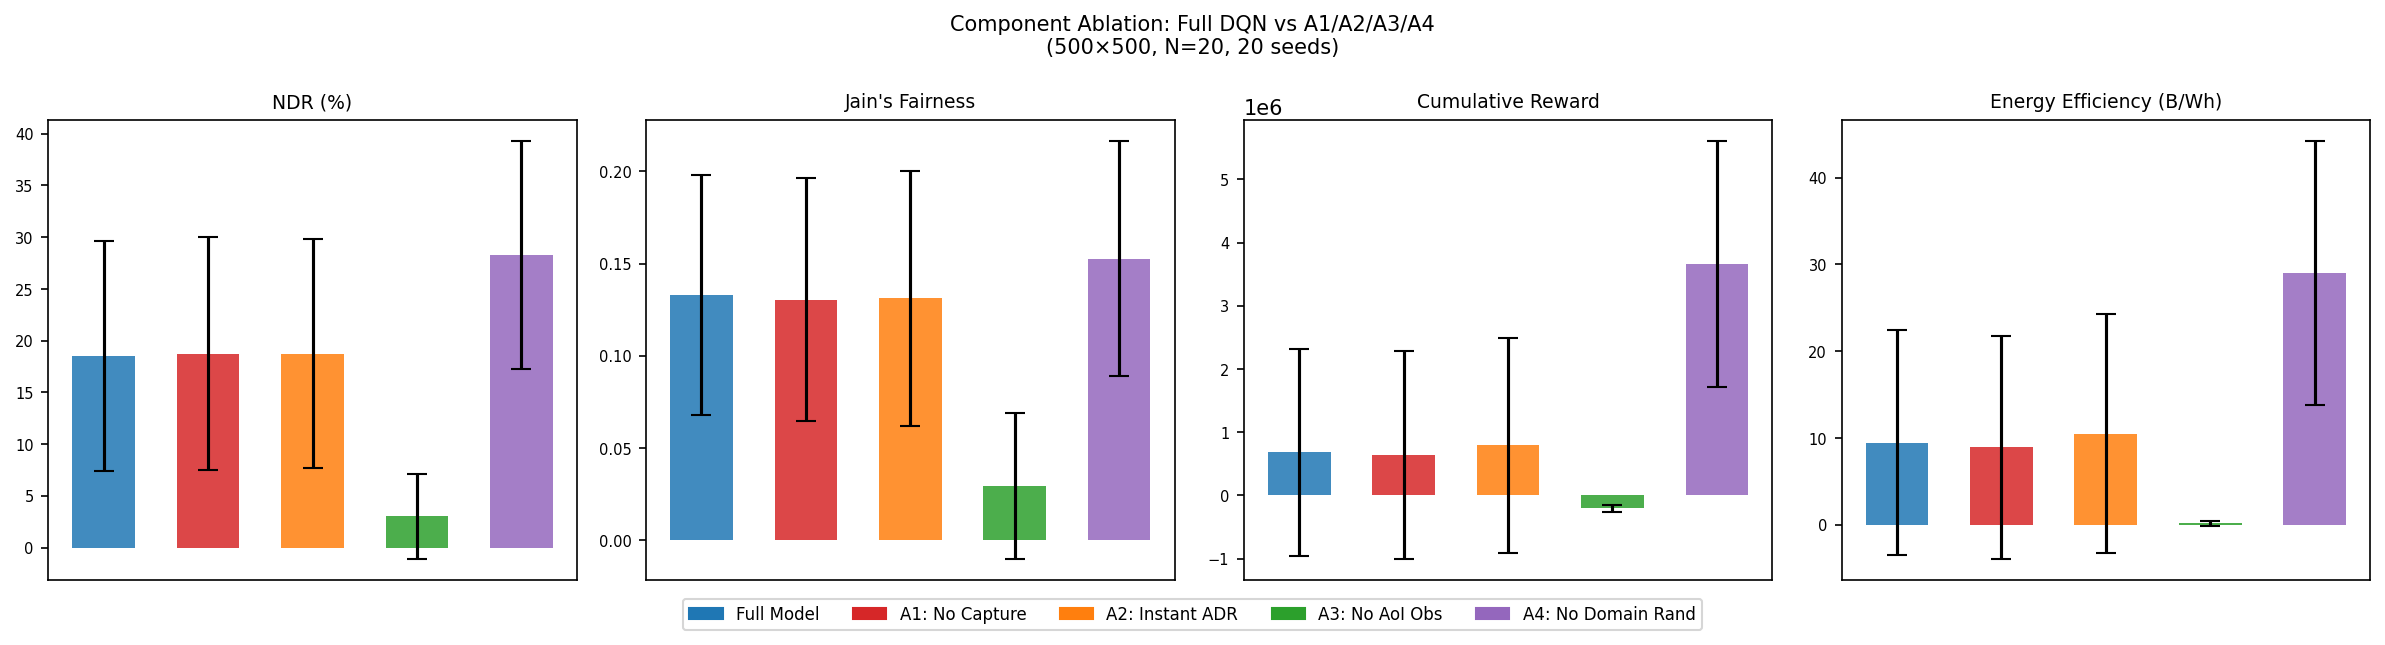
\includegraphics[width=0.92\textwidth]{../src/agents/dqn/dqn_evaluation_results/baseline_results/ablation_comparison.png}
    \caption{Component ablation bars. Full Model versus the four
    ablation conditions (Capture Effect removed, instant ADR, AoI
    zeroed, fixed environment) across cumulative reward, NDR, Jain's
    fairness index, and energy efficiency. Regenerable from
    \texttt{ablation\_study.py}.}
    \label{fig:ablation_bars}
\end{figure}

\subsection*{Multi-Seed Pareto and Radar Views}

\begin{figure}[H]
    \centering
    \begin{subfigure}[b]{0.48\textwidth}
        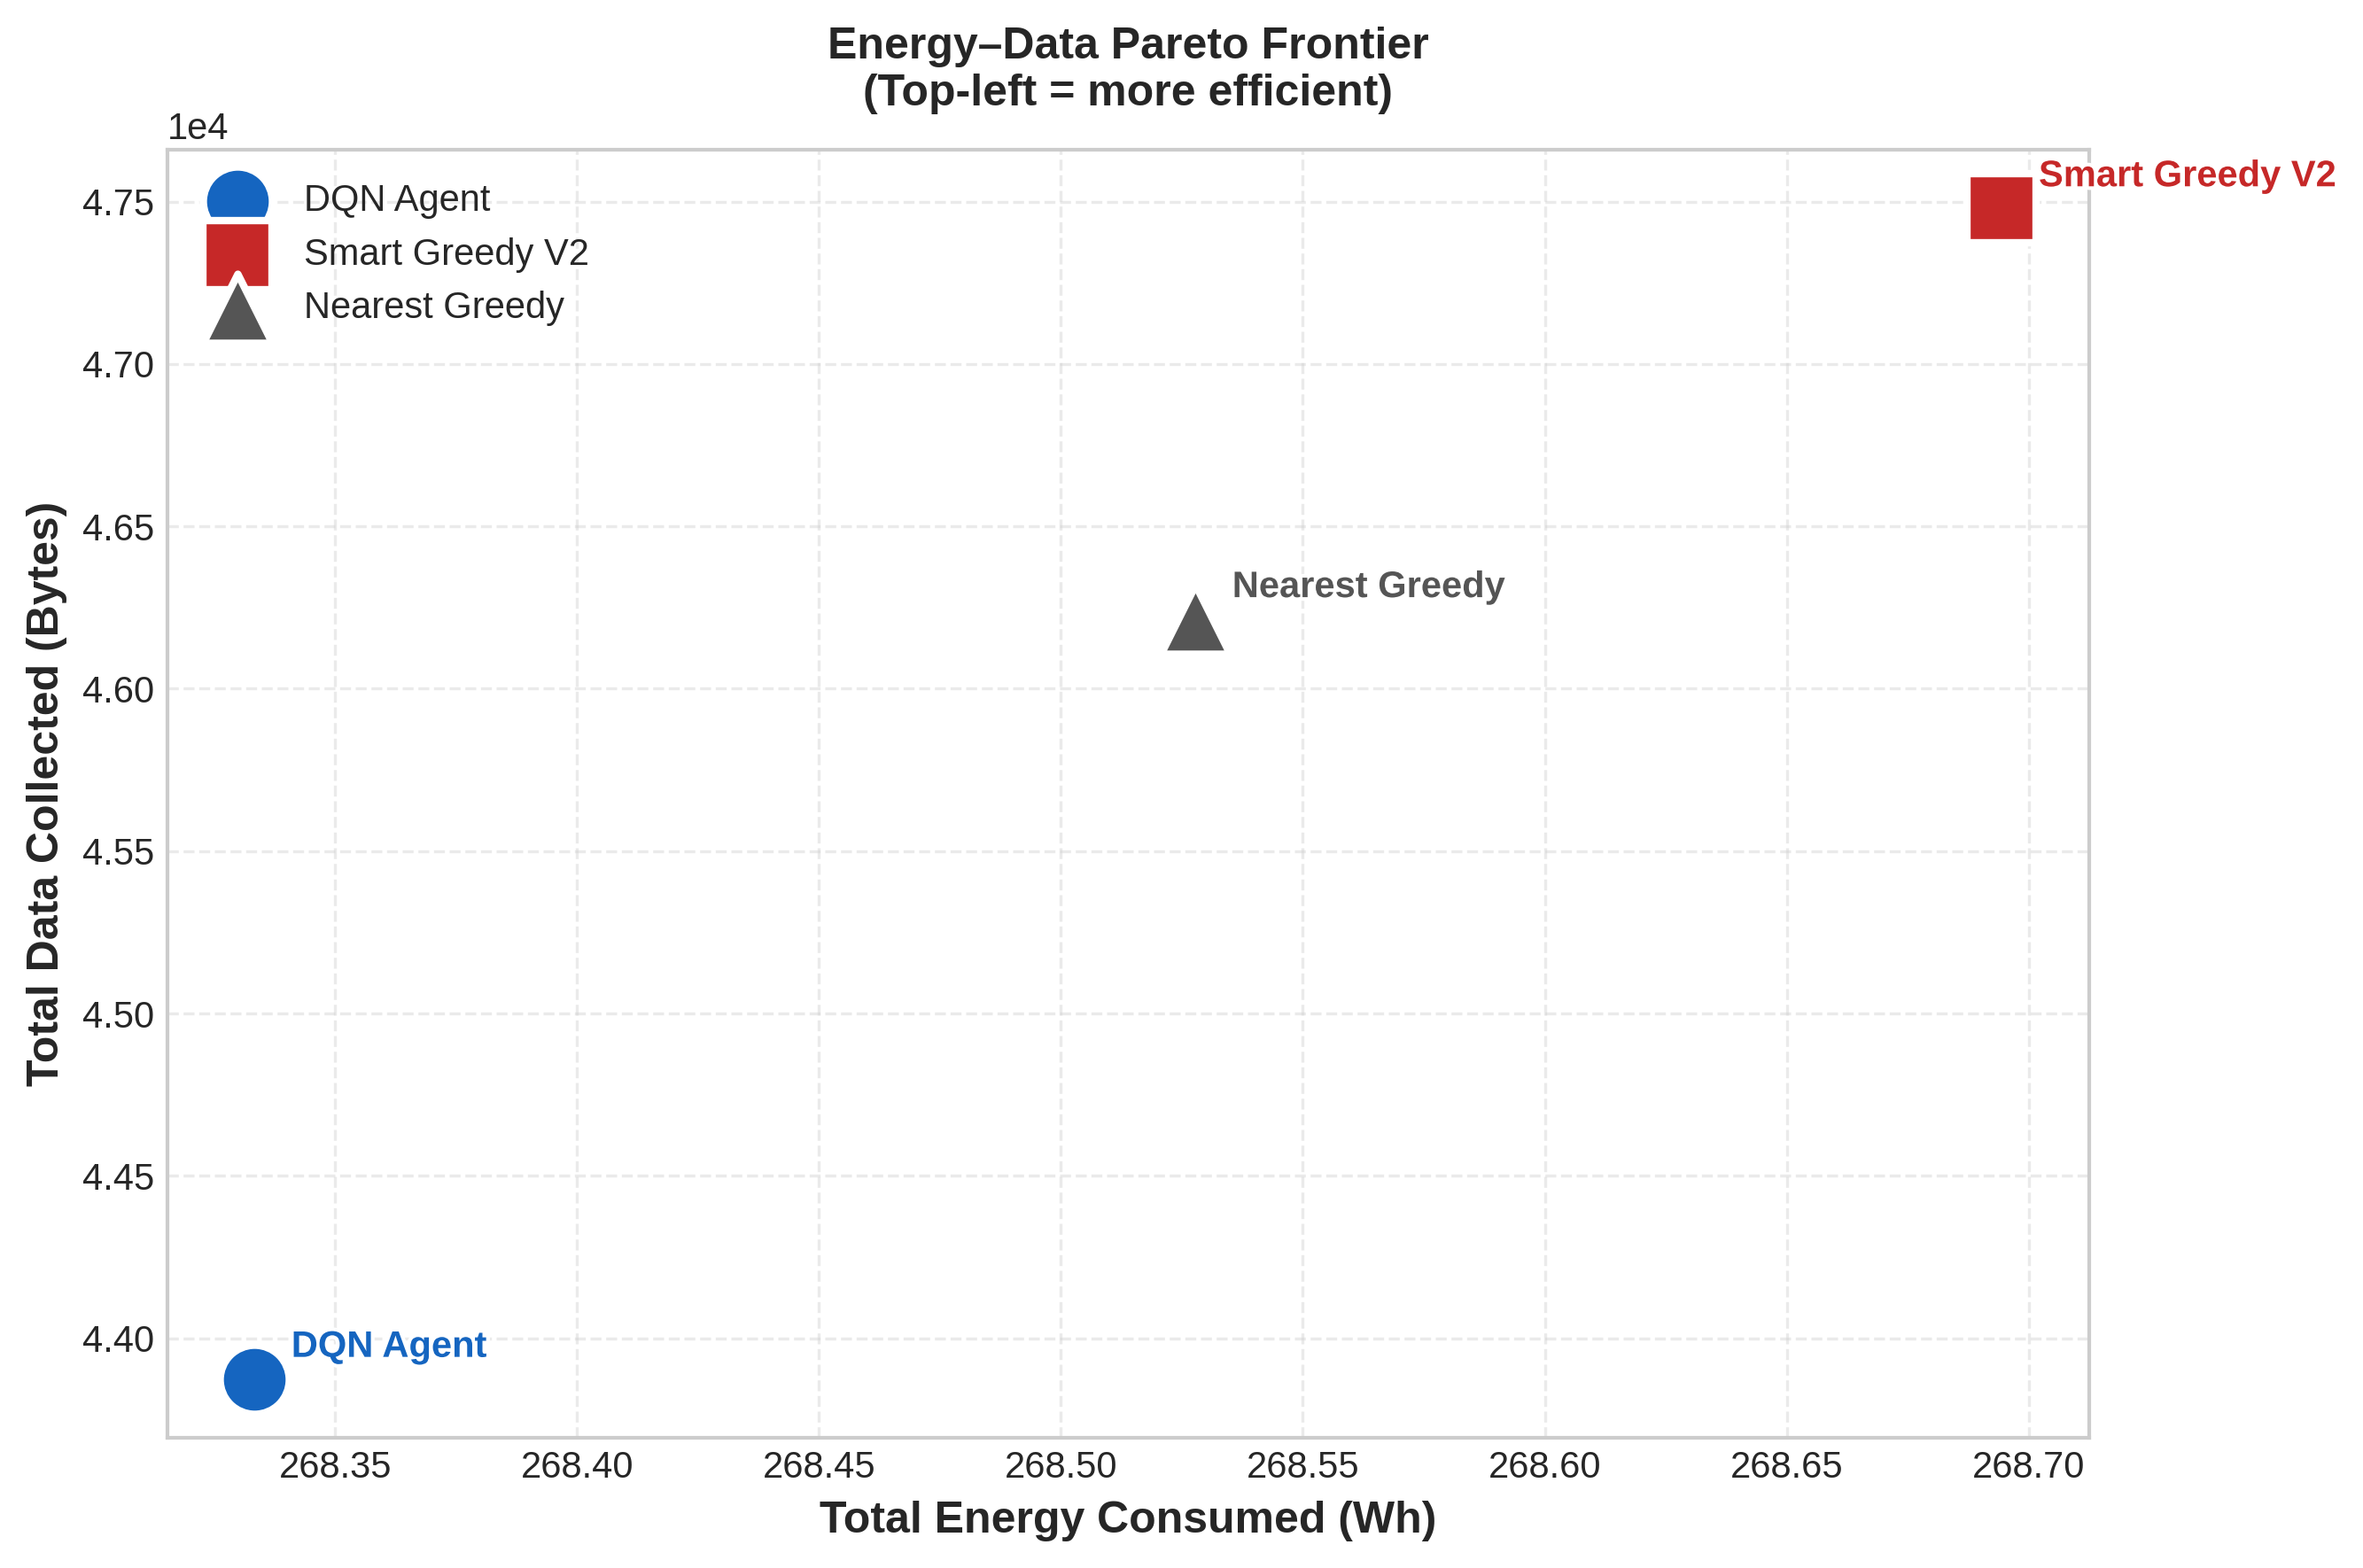
\includegraphics[width=\textwidth]{../src/agents/dqn/dqn_evaluation_results/baseline_results/pareto_scatter.png}
        \caption{Reward vs energy efficiency.}
    \end{subfigure}
    \hfill
    \begin{subfigure}[b]{0.48\textwidth}
        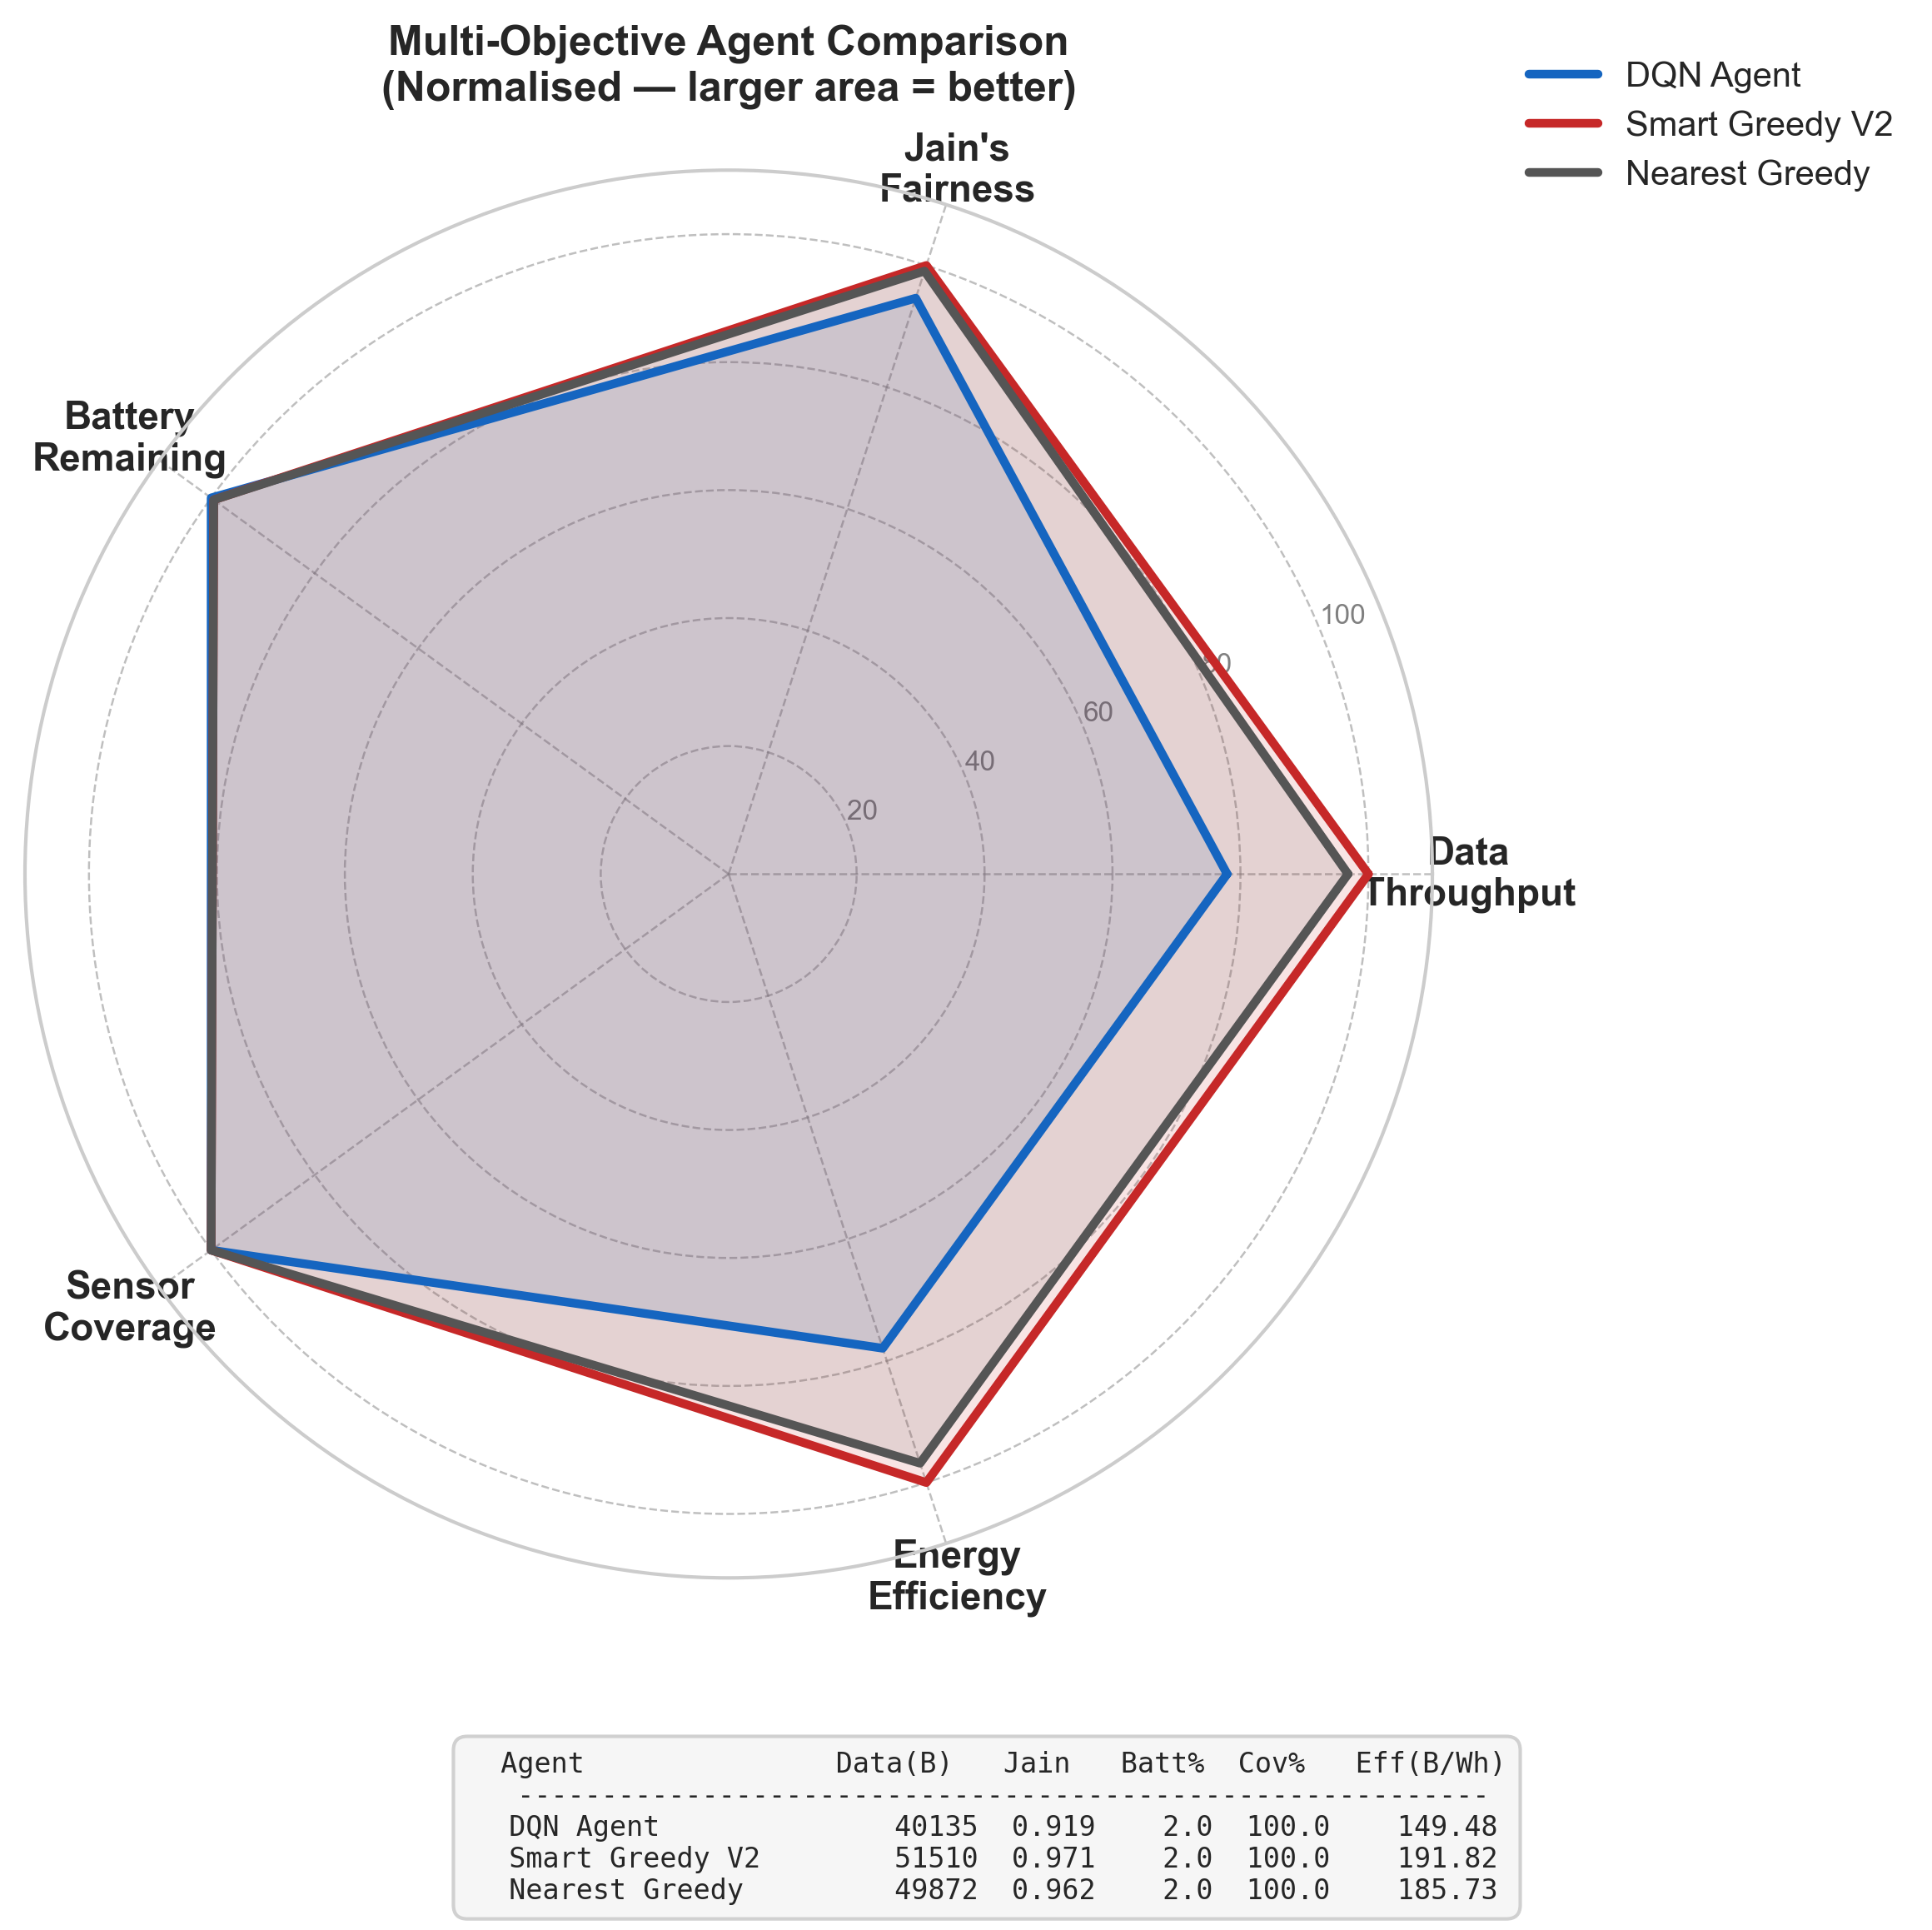
\includegraphics[width=\textwidth]{../src/agents/dqn/dqn_evaluation_results/baseline_results/radar_chart.png}
        \caption{Multi-metric radar.}
    \end{subfigure}
    \caption{The same five-condition scalability data from
    Figure~\ref{fig:scalability_combined}, plotted as a Pareto scatter
    (reward vs energy efficiency) and a multi-metric radar.
    Same 50-seed results, different layout.}
    \label{fig:pareto_radar}
\end{figure}

\subsection*{Fairness Heatmap}

\begin{figure}[H]
    \centering
    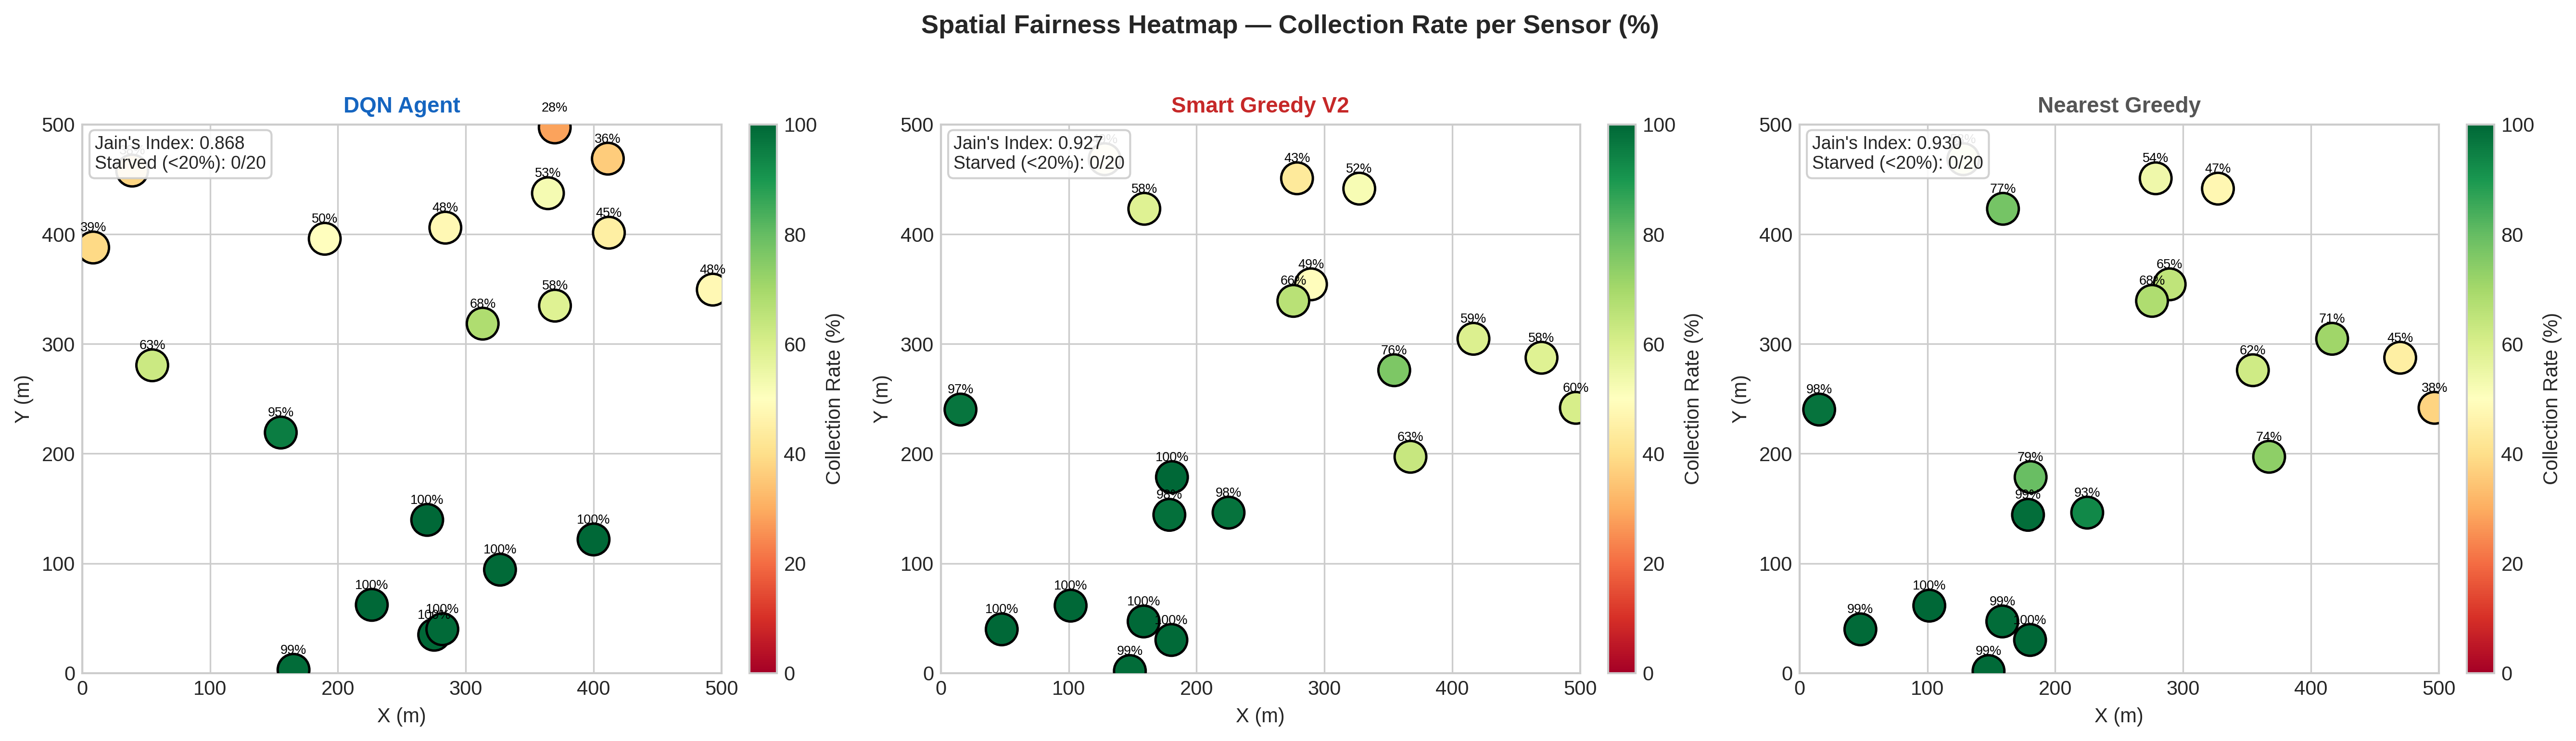
\includegraphics[width=0.85\textwidth]{../src/agents/dqn/dqn_evaluation_results/baseline_results/fairness_heatmap.png}
    \caption{Per-sensor collection fairness heatmap (rows: sensors,
    columns: agents). Darker cells indicate higher fraction of the
    sensor's total data successfully collected.}
    \label{fig:fairness_heatmap}
\end{figure}

\subsection*{Lawnmower Indicative Results}

The Lawnmower baseline was run at 5 seeds, not 50; per-episode reward
and per-metric traces are in \texttt{baseline\_results/lawnmower\_results.csv}.
At $200{\times}200$, $N{=}50$ it achieves $98\%$ coverage with cumulative
reward roughly $78\%$ of the DQN's on the matched seed. It is a
coverage-only indicator and is not included in the statistical comparisons
in the main body.
 % A.10 Additional Figures
		\input{appendices/extended_methodology} % A.11 Extended Methodology
		\input{appendices/extended_results}     % A.12 Extended Results
	\end{uomappendix}

	%%%%%%%%%%%%%%%%%% END MATTER %%%%%%%%%%%%%%%%%%
\end{document}